%%%%%%%%%%%%%%%%%%%%%%%%%%%%%%%%%%%%%%%%%
% The Legrand Orange Book
% LaTeX Template
% Version 2.1 (14/11/15)
%
% This template has been downloaded from:
% http://www.LaTeXTemplates.com
%
% Mathias Legrand (legrand.mathias@gmail.com) with modifications by:
% Vel (vel@latextemplates.com)
%
% License:
% CC BY-NC-SA 3.0 (http://creativecommons.org/licenses/by-nc-sa/3.0/)
%
% Compiling this template:
% This template uses biber for its bibliography and makeindex for its index.
% When you first open the template, compile it from the command line with the 
% commands below to make sure your LaTeX distribution is configured correctly:
%
% 1) pdflatex main
% 2) makeindex main.idx -s StyleInd.ist
% 3) biber main
% 4) pdflatex main x 2
%
% After this, when you wish to update the bibliography/index use the appropriate
% command above and make sure to compile with pdflatex several times 
% afterwards to propagate your changes to the document.
%
% This template also uses a number of packages which may need to be
% updated to the newest versions for the template to compile. It is strongly
% recommended you update your LaTeX distribution if you have any
% compilation errors.
%
% Important note:
% Chapter heading images should have a 2:1 width:height ratio,
% e.g. 920px width and 460px height.
%
%%%%%%%%%%%%%%%%%%%%%%%%%%%%%%%%%%%%%%%%%

%----------------------------------------------------------------------------------------
%	PACKAGES AND OTHER DOCUMENT CONFIGURATIONS
%----------------------------------------------------------------------------------------

\documentclass[12pt,fleqn]{book} % Default font size and left-justified equations

%----------------------------------------------------------------------------------------

%%%%%%%%%%%%%%%%%%%%%%%%%%%%%%%%%%%%%%%%%
%% THIS FILE HAS BEEN MODIFIED FOR USE IN STELLARIUM
% The Legrand Orange Book
% Structural Definitions File
% Version 2.0 (9/2/15)
%
% Original author:
% Mathias Legrand (legrand.mathias@gmail.com) with modifications by:
% Vel (vel@latextemplates.com)
% 
% This file has been downloaded from:
% http://www.LaTeXTemplates.com
%
% License:
% CC BY-NC-SA 3.0 (http://creativecommons.org/licenses/by-nc-sa/3.0/)
%
%%%%%%%%%%%%%%%%%%%%%%%%%%%%%%%%%%%%%%%%%

%----------------------------------------------------------------------------------------
%	VARIOUS REQUIRED PACKAGES AND CONFIGURATIONS
%----------------------------------------------------------------------------------------

\usepackage[top=3cm,bottom=3cm,left=3cm,right=3cm,headsep=10pt,a4paper]{geometry} % Page margins

\usepackage{graphicx} % Required for including pictures
\graphicspath{{pictures/}} % Specifies the directory where pictures are stored

\usepackage{tikz} % Required for drawing custom shapes
\usepackage{longtable}
\usepackage{tabularx}
\usepackage{tabu}
\usepackage{gensymb}
\usepackage[english]{babel} % English language/hyphenation

\usepackage{enumitem} % Customize lists
\setlist{nolistsep} % Reduce spacing between bullet points and numbered lists

\usepackage{booktabs} % Required for nicer horizontal rules in tables

\usepackage{xcolor} % Required for specifying colors by name
\definecolor{ocre}{RGB}{51,153,255} % Define the color used for highlighting throughout the book

\usepackage{color}
\usepackage{listings}

%----------------------------------------------------------------------------------------
%	NEW COMMANDS AND ADDITIONS
%----------------------------------------------------------------------------------------

% Emergency definition as this is not in MiKTeX.
\makeatletter
%\DeclareRobustCommand*
\providecommand\textsubscript[1]{%
  \@textsubscript{\selectfont#1}}
\def\@textsubscript#1{%
  {\m@th\ensuremath{_{\mbox{\fontsize\sf@size\z@#1}}}}}
\makeatother

\usepackage{newunicodechar}
\newunicodechar{°}{\degree}

%% GZ: some typesetting macros given here once are better than immediate formatting.

%% File names. 
\newcommand{\file}[1]{\texttt{#1}}
%% console commands, CLI arguments, etc.
\newcommand{\command}[1]{\texttt{#1}}
%% Keypress buttons. This is just a font change now, but can be a boxed key or such.
\newcommand{\key}[1]{\textbf{\textsf{#1}}}
%% Person names. In some places they have been italicised, in others bold. Make them appear the same with this, and add them to the index:
\newcommand{\name}[1]{\textsc{#1}\index{#1}}
%% Some new term that is presented here with emphasis and also goes immediately to the index. 
\newcommand{\indexterm}[1]{\emph{#1}\index{#1}}

%% A command to show the version number when a feature was introduced in the margin. Give only the version number. TODO Decide on formatting etc.
\newcommand{\newFeature}[1]{\marginpar{#1}}

%% A few units. Add what you need in the same style here.
\newcommand{\cm}{\ensuremath{\,\mathrm{cm}}}
\newcommand{\mm}{\ensuremath{\,\mathrm{mm}}}
\newcommand{\km}{\ensuremath{\,\mathrm{km}}}
\newcommand{\um}{\ensuremath{\,\mathrm{\mu m}}}
\newcommand{\AU}{\ensuremath{\,\mathrm{AU}}}
\newcommand{\LY}{\ensuremath{\,\mathrm{LY}}}
\newcommand{\pc}{\ensuremath{\,\mathrm{pc}}}
\newcommand{\kpc}{\ensuremath{\,\mathrm{kpc}}}
\newcommand{\Mpc}{\ensuremath{\,\mathrm{Mpc}}}
\newcommand{\Hz}{\ensuremath{\,\mathrm{Hz}}}
\newcommand{\MHz}{\ensuremath{\,\mathrm{MHz}}}
\newcommand{\mJy}{\ensuremath{\,\mathrm{mJy}}}
\newcommand{\kg}{\ensuremath{\,\mathrm{kg}}}
\newcommand{\g}{\ensuremath{\,\mathrm{g}}}

\lstnewenvironment{commands}{\lstset{language=sh,basicstyle=\ttfamily\small,%
                                     backgroundcolor=\color{black!5},frame=leftline,rulecolor=\color{blue},framerule=1pt}%
                             }{}%
\lstnewenvironment{configfile}{\lstset{language=sh,basicstyle=\ttfamily\small,%
                                   backgroundcolor=\color{black!5},frame=shadowbox,rulecolor=\color{blue},framerule=1pt}%
                             }{}%


%% Allow chapter authors where this seems appropriate.
%% From http://tex.stackexchange.com/questions/156862/displaying-author-for-each-chapter-in-book
\usepackage{suffix}

\newcommand\chapterauthor[1]{\authortoc{#1}\printchapterauthor{#1}}
\WithSuffix\newcommand\chapterauthor*[1]{\printchapterauthor{#1}}

\makeatletter
\newcommand{\printchapterauthor}[1]{%
  {\parindent0pt\vspace*{-25pt}%
  \linespread{1.1}\large\scshape#1%
  \par\nobreak\vspace*{35pt}}
  \@afterheading%
}
\newcommand{\authortoc}[1]{%
  \addtocontents{toc}{\vskip-10pt}%
  \addtocontents{toc}{%
    \protect\contentsline{chapter}%
    {\hskip1.3em\mdseries\scshape\protect\scriptsize#1}{}{}}
  \addtocontents{toc}{\vskip5pt}%
}
\makeatother

%----------------------------------------------------------------------------------------
%	FONTS
%----------------------------------------------------------------------------------------

\usepackage{avant} % Use the Avantgarde font for headings
%\usepackage{times} % Use the Times font for headings
\usepackage{mathptmx} % Use the Adobe Times Roman as the default text font together with math symbols from the Symbol, Chancery and Computer Modern fonts

\usepackage{microtype} % Slightly tweak font spacing for aesthetics
\usepackage[utf8]{inputenc} % Required for including letters with accents
\usepackage[T1]{fontenc} % Use 8-bit encoding that has 256 glyphs

%----------------------------------------------------------------------------------------
%	BIBLIOGRAPHY AND INDEX
%----------------------------------------------------------------------------------------

\usepackage[style=alphabetic,citestyle=numeric,sorting=nyt,sortcites=true,autopunct=true,babel=hyphen,hyperref=true,abbreviate=false,backref=true,backend=biber]{biblatex}
\addbibresource{bibliography.bib} % BibTeX bibliography file
\defbibheading{bibempty}{}

\usepackage{calc} % For simpler calculation - used for spacing the index letter headings correctly
\usepackage{makeidx} % Required to make an index
\makeindex % Tells LaTeX to create the files required for indexing

%----------------------------------------------------------------------------------------
%	MAIN TABLE OF CONTENTS
%----------------------------------------------------------------------------------------

\usepackage{titletoc} % Required for manipulating the table of contents

\contentsmargin{0cm} % Removes the default margin

% Part text styling
\titlecontents{part}[0cm]
{\addvspace{20pt}\centering\large\bfseries}
{}
{}
{}

% Chapter text styling
\titlecontents{chapter}[1.35cm] % Indentation
{\addvspace{12pt}\large\sffamily\bfseries} % Spacing and font options for chapters
{\color{ocre!60}\contentslabel[\Large\thecontentslabel]{1.35cm}\color{ocre}} % Chapter number
{\color{ocre}}  
{\color{ocre!60}\normalsize\;\titlerule*[.5pc]{.}\;\thecontentspage} % Page number

% Section text styling
\titlecontents{section}[1.35cm] % Indentation
{\addvspace{3pt}\sffamily\bfseries} % Spacing and font options for sections
{\contentslabel[\thecontentslabel]{1.35cm}} % Section number
{}
{\hfill\color{black}\thecontentspage} % Page number
[]

% Subsection text styling
\titlecontents{subsection}[1.35cm] % Indentation
{\addvspace{1pt}\sffamily\small} % Spacing and font options for subsections
{\contentslabel[\thecontentslabel]{1.35cm}} % Subsection number
{}
{\ \titlerule*[.5pc]{.}\;\thecontentspage} % Page number
[]

% List of figures
\titlecontents{figure}[0em]
{\addvspace{-5pt}\sffamily}
{\thecontentslabel\hspace*{1em}}
{}
{\ \titlerule*[.5pc]{.}\;\thecontentspage}
[]

% List of tables
\titlecontents{table}[0em]
{\addvspace{-5pt}\sffamily}
{\thecontentslabel\hspace*{1em}}
{}
{\ \titlerule*[.5pc]{.}\;\thecontentspage}
[]

%----------------------------------------------------------------------------------------
%	MINI TABLE OF CONTENTS IN PART HEADS
%----------------------------------------------------------------------------------------

% Chapter text styling
\titlecontents{lchapter}[0em] % Indenting
{\addvspace{15pt}\large\sffamily\bfseries} % Spacing and font options for chapters
{\color{ocre}\contentslabel[\Large\thecontentslabel]{1.25cm}\color{ocre}} % Chapter number
{}  
{\color{ocre}\normalsize\sffamily\bfseries\;\titlerule*[.5pc]{.}\;\thecontentspage} % Page number

% Section text styling
\titlecontents{lsection}[0em] % Indenting
{\sffamily\small} % Spacing and font options for sections
{\contentslabel[\thecontentslabel]{1.25cm}} % Section number
{}
{}

% Subsection text styling
\titlecontents{lsubsection}[.5em] % Indentation
{\normalfont\footnotesize\sffamily} % Font settings
{}
{}
{}

%----------------------------------------------------------------------------------------
%	PAGE HEADERS
%----------------------------------------------------------------------------------------

\usepackage{fancyhdr} % Required for header and footer configuration

\pagestyle{fancy}
\renewcommand{\chaptermark}[1]{\markboth{\sffamily\normalsize\bfseries\chaptername\ \thechapter.\ #1}{}} % Chapter text font settings
\renewcommand{\sectionmark}[1]{\markright{\sffamily\normalsize\thesection\hspace{5pt}#1}{}} % Section text font settings
\fancyhf{} \fancyhead[LE,RO]{\sffamily\normalsize\thepage} % Font setting for the page number in the header
\fancyhead[LO]{\rightmark} % Print the nearest section name on the left side of odd pages
\fancyhead[RE]{\leftmark} % Print the current chapter name on the right side of even pages
\renewcommand{\headrulewidth}{0.5pt} % Width of the rule under the header
\addtolength{\headheight}{2.5pt} % Increase the spacing around the header slightly
\renewcommand{\footrulewidth}{0pt} % Removes the rule in the footer
\fancypagestyle{plain}{\fancyhead{}\renewcommand{\headrulewidth}{0pt}} % Style for when a plain pagestyle is specified

% Removes the header from odd empty pages at the end of chapters
\makeatletter
\renewcommand{\cleardoublepage}{
\clearpage\ifodd\c@page\else
\hbox{}
\vspace*{\fill}
\thispagestyle{empty}
\newpage
\fi}

%----------------------------------------------------------------------------------------
%	THEOREM STYLES
%----------------------------------------------------------------------------------------

\usepackage{amsmath,amsfonts,amssymb,amsthm} % For math equations, theorems, symbols, etc

\newcommand{\intoo}[2]{\mathopen{]}#1\,;#2\mathclose{[}}
\newcommand{\ud}{\mathop{\mathrm{{}d}}\mathopen{}}
\newcommand{\intff}[2]{\mathopen{[}#1\,;#2\mathclose{]}}
\newtheorem{notation}{Notation}[chapter]

% Boxed/framed environments
\newtheoremstyle{ocrenumbox}% % Theorem style name
{0pt}% Space above
{0pt}% Space below
{\normalfont}% % Body font
{}% Indent amount
{\small\bf\sffamily\color{ocre}}% % Theorem head font
{\;}% Punctuation after theorem head
{0.25em}% Space after theorem head
{\small\sffamily\color{ocre}\thmname{#1}\nobreakspace\thmnumber{\@ifnotempty{#1}{}\@upn{#2}}% Theorem text (e.g. Theorem 2.1)
\thmnote{\nobreakspace\the\thm@notefont\sffamily\bfseries\color{black}---\nobreakspace#3.}} % Optional theorem note
\renewcommand{\qedsymbol}{$\blacksquare$}% Optional qed square

\newtheoremstyle{blacknumex}% Theorem style name
{5pt}% Space above
{5pt}% Space below
{\normalfont}% Body font
{} % Indent amount
{\small\bf\sffamily}% Theorem head font
{\;}% Punctuation after theorem head
{0.25em}% Space after theorem head
{\small\sffamily{\tiny\ensuremath{\blacksquare}}\nobreakspace\thmname{#1}\nobreakspace\thmnumber{\@ifnotempty{#1}{}\@upn{#2}}% Theorem text (e.g. Theorem 2.1)
\thmnote{\nobreakspace\the\thm@notefont\sffamily\bfseries---\nobreakspace#3.}}% Optional theorem note

\newtheoremstyle{blacknumbox} % Theorem style name
{0pt}% Space above
{0pt}% Space below
{\normalfont}% Body font
{}% Indent amount
{\small\bf\sffamily}% Theorem head font
{\;}% Punctuation after theorem head
{0.25em}% Space after theorem head
{\small\sffamily\thmname{#1}\nobreakspace\thmnumber{\@ifnotempty{#1}{}\@upn{#2}}% Theorem text (e.g. Theorem 2.1)
\thmnote{\nobreakspace\the\thm@notefont\sffamily\bfseries---\nobreakspace#3.}}% Optional theorem note

% Non-boxed/non-framed environments
\newtheoremstyle{ocrenum}% % Theorem style name
{5pt}% Space above
{5pt}% Space below
{\normalfont}% % Body font
{}% Indent amount
{\small\bf\sffamily\color{ocre}}% % Theorem head font
{\;}% Punctuation after theorem head
{0.25em}% Space after theorem head
{\small\sffamily\color{ocre}\thmname{#1}\nobreakspace\thmnumber{\@ifnotempty{#1}{}\@upn{#2}}% Theorem text (e.g. Theorem 2.1)
\thmnote{\nobreakspace\the\thm@notefont\sffamily\bfseries\color{black}---\nobreakspace#3.}} % Optional theorem note
\renewcommand{\qedsymbol}{$\blacksquare$}% Optional qed square
\makeatother

% Defines the theorem text style for each type of theorem to one of the three styles above
\newcounter{dummy} 
\numberwithin{dummy}{section}
\theoremstyle{ocrenumbox}
\newtheorem{theoremeT}[dummy]{Theorem}
\newtheorem{problem}{Problem}[chapter]
\newtheorem{exerciseT}{Exercise}[chapter]
\theoremstyle{blacknumex}
\newtheorem{exampleT}{Example}[chapter]
\theoremstyle{blacknumbox}
\newtheorem{vocabulary}{Vocabulary}[chapter]
\newtheorem{definitionT}{Definition}[section]
\newtheorem{corollaryT}[dummy]{Corollary}
\theoremstyle{ocrenum}
\newtheorem{proposition}[dummy]{Proposition}

%----------------------------------------------------------------------------------------
%	DEFINITION OF COLORED BOXES
%----------------------------------------------------------------------------------------

\RequirePackage[framemethod=default]{mdframed} % Required for creating the theorem, definition, exercise and corollary boxes

% Theorem box
\newmdenv[skipabove=7pt,
skipbelow=7pt,
backgroundcolor=black!5,
linecolor=ocre,
innerleftmargin=5pt,
innerrightmargin=5pt,
innertopmargin=5pt,
leftmargin=0cm,
rightmargin=0cm,
innerbottommargin=5pt]{tBox}

% Config box
\newmdenv[skipabove=7pt,
skipbelow=7pt,
rightline=false,
leftline=true,
topline=false,
bottomline=false,
backgroundcolor=black!5,
linecolor=ocre,
innerleftmargin=5pt,
innerrightmargin=5pt,
innertopmargin=5pt,
innerbottommargin=5pt,
leftmargin=0cm,
rightmargin=0cm,
linewidth=1pt]{wBox}

% Exercise box	  
\newmdenv[skipabove=7pt,
skipbelow=7pt,
rightline=false,
leftline=true,
topline=false,
bottomline=false,
backgroundcolor=ocre!10,
linecolor=ocre,
innerleftmargin=5pt,
innerrightmargin=5pt,
innertopmargin=5pt,
innerbottommargin=5pt,
leftmargin=0cm,
rightmargin=0cm,
linewidth=4pt]{eBox}	

% Definition box
\newmdenv[skipabove=7pt,
skipbelow=7pt,
rightline=false,
leftline=true,
topline=false,
bottomline=false,
linecolor=ocre,
innerleftmargin=5pt,
innerrightmargin=5pt,
innertopmargin=0pt,
leftmargin=0cm,
rightmargin=0cm,
linewidth=4pt,
innerbottommargin=0pt]{dBox}	

% Corollary box
\newmdenv[skipabove=7pt,
skipbelow=7pt,
rightline=false,
leftline=true,
topline=false,
bottomline=false,
linecolor=gray,
backgroundcolor=black!5,
innerleftmargin=5pt,
innerrightmargin=5pt,
innertopmargin=5pt,
leftmargin=0cm,
rightmargin=0cm,
linewidth=4pt,
innerbottommargin=5pt]{cBox}

% Creates an environment for each type of theorem and assigns it a theorem text style from the "Theorem Styles" section above and a colored box from above
\newenvironment{theorem}{\begin{tBox}\begin{theoremeT}}{\end{theoremeT}\end{tBox}}
\newenvironment{exercise}{\begin{eBox}\begin{exerciseT}}{\hfill{\color{ocre}\tiny\ensuremath{\blacksquare}}\end{exerciseT}\end{eBox}}				  
\newenvironment{definition}{\begin{dBox}\begin{definitionT}}{\end{definitionT}\end{dBox}}	
\newenvironment{example}{\begin{exampleT}}{\hfill{\tiny\ensuremath{\blacksquare}}\end{exampleT}}		
\newenvironment{corollary}{\begin{cBox}\begin{corollaryT}}{\end{corollaryT}\end{cBox}}	
\newenvironment{config}{\begin{wBox}}{\end{wBox}}

%----------------------------------------------------------------------------------------
%	REMARK ENVIRONMENT
%----------------------------------------------------------------------------------------

\newenvironment{remark}{\par\vspace{10pt}\small % Vertical white space above the remark and smaller font size
\begin{list}{}{
\leftmargin=35pt % Indentation on the left
\rightmargin=25pt}\item\ignorespaces % Indentation on the right
\makebox[-2.5pt]{\begin{tikzpicture}[overlay]
\node[draw=ocre!60,line width=1pt,circle,fill=ocre!25,font=\sffamily\bfseries,inner sep=2pt,outer sep=0pt] at (-15pt,0pt){\textcolor{ocre}{R}};\end{tikzpicture}} % Orange R in a circle
\advance\baselineskip -1pt}{\end{list}\vskip5pt} % Tighter line spacing and white space after remark

%----------------------------------------------------------------------------------------
%	SECTION NUMBERING IN THE MARGIN
%----------------------------------------------------------------------------------------

\makeatletter
\renewcommand{\@seccntformat}[1]{\llap{\textcolor{ocre}{\csname the#1\endcsname}\hspace{1em}}}                    
\renewcommand{\section}{\@startsection{section}{1}{\z@}
{-4ex \@plus -1ex \@minus -.4ex}
{1ex \@plus.2ex }
{\normalfont\large\sffamily\bfseries}}
\renewcommand{\subsection}{\@startsection {subsection}{2}{\z@}
{-3ex \@plus -0.1ex \@minus -.4ex}
{0.5ex \@plus.2ex }
{\normalfont\sffamily\bfseries}}
\renewcommand{\subsubsection}{\@startsection {subsubsection}{3}{\z@}
{-2ex \@plus -0.1ex \@minus -.2ex}
{.2ex \@plus.2ex }
{\normalfont\small\sffamily\bfseries}}                        
\renewcommand\paragraph{\@startsection{paragraph}{4}{\z@}
{-2ex \@plus-.2ex \@minus .2ex}
{.1ex}
{\normalfont\small\sffamily\bfseries}}

%----------------------------------------------------------------------------------------
%	PART HEADINGS
%----------------------------------------------------------------------------------------

% numbered part in the table of contents
\newcommand{\@mypartnumtocformat}[2]{%
\setlength\fboxsep{0pt}%
\noindent\colorbox{ocre!20}{\strut\parbox[c][.7cm]{\ecart}{\color{ocre!70}\Large\sffamily\bfseries\centering#1}}\hskip\esp\colorbox{ocre!40}{\strut\parbox[c][.7cm]{\linewidth-\ecart-\esp}{\Large\sffamily\centering#2}}}%
%%%%%%%%%%%%%%%%%%%%%%%%%%%%%%%%%%
% unnumbered part in the table of contents
\newcommand{\@myparttocformat}[1]{%
\setlength\fboxsep{0pt}%
\noindent\colorbox{ocre!40}{\strut\parbox[c][.7cm]{\linewidth}{\Large\sffamily\centering#1}}}%
%%%%%%%%%%%%%%%%%%%%%%%%%%%%%%%%%%
\newlength\esp
\setlength\esp{4pt}
\newlength\ecart
\setlength\ecart{1.2cm-\esp}
\newcommand{\thepartimage}{}%
\newcommand{\partimage}[1]{\renewcommand{\thepartimage}{#1}}%
\def\@part[#1]#2{%
\ifnum \c@secnumdepth >-2\relax%
\refstepcounter{part}%
\addcontentsline{toc}{part}{\texorpdfstring{\protect\@mypartnumtocformat{\thepart}{#1}}{\partname~\thepart\ ---\ #1}}
\else%
\addcontentsline{toc}{part}{\texorpdfstring{\protect\@myparttocformat{#1}}{#1}}%
\fi%
\startcontents%
\markboth{}{}%
{\thispagestyle{empty}%
\begin{tikzpicture}[remember picture,overlay]%
\node at (current page.north west){\begin{tikzpicture}[remember picture,overlay]%	
\fill[ocre!20](0cm,0cm) rectangle (\paperwidth,-\paperheight);
\node[anchor=north] at (4cm,-3.25cm){\color{ocre!40}\fontsize{220}{100}\sffamily\bfseries\@Roman\c@part}; 
\node[anchor=south east] at (\paperwidth-1cm,-\paperheight+1cm){\parbox[t][][t]{8.5cm}{
\printcontents{l}{0}{\setcounter{tocdepth}{1}}%
}};
\node[anchor=north east] at (\paperwidth-1.5cm,-3.25cm){\parbox[t][][t]{15cm}{\strut\raggedleft\color{white}\fontsize{30}{30}\sffamily\bfseries#2}};
\end{tikzpicture}};
\end{tikzpicture}}%
\@endpart}
\def\@spart#1{%
\startcontents%
\phantomsection
{\thispagestyle{empty}%
\begin{tikzpicture}[remember picture,overlay]%
\node at (current page.north west){\begin{tikzpicture}[remember picture,overlay]%	
\fill[ocre!20](0cm,0cm) rectangle (\paperwidth,-\paperheight);
\node[anchor=north east] at (\paperwidth-1.5cm,-3.25cm){\parbox[t][][t]{15cm}{\strut\raggedleft\color{white}\fontsize{30}{30}\sffamily\bfseries#1}};
\end{tikzpicture}};
\end{tikzpicture}}
\addcontentsline{toc}{part}{\texorpdfstring{%
\setlength\fboxsep{0pt}%
\noindent\protect\colorbox{ocre!40}{\strut\protect\parbox[c][.7cm]{\linewidth}{\Large\sffamily\protect\centering #1\quad\mbox{}}}}{#1}}%
\@endpart}
\def\@endpart{\vfil\newpage
\if@twoside
\if@openright
\null
\thispagestyle{empty}%
\newpage
\fi
\fi
\if@tempswa
\twocolumn
\fi}

%----------------------------------------------------------------------------------------
%	CHAPTER HEADINGS
%----------------------------------------------------------------------------------------

\newcommand{\thechapterimage}{}%
\newcommand{\chapterimage}[1]{\renewcommand{\thechapterimage}{#1}}%
\def\@makechapterhead#1{%
{\parindent \z@ \raggedright \normalfont
\ifnum \c@secnumdepth >\m@ne
\if@mainmatter
\begin{tikzpicture}[remember picture,overlay]
\node at (current page.north west)
{\begin{tikzpicture}[remember picture,overlay]
\node[anchor=north west,inner sep=0pt] at (0,0) {\includegraphics[width=\paperwidth]{\thechapterimage}};
\draw[anchor=west] (\Gm@lmargin,-9cm) node [line width=2pt,rounded corners=15pt,draw=ocre,fill=white,fill opacity=0.5,inner sep=15pt]{\strut\makebox[22cm]{}};
\draw[anchor=west] (\Gm@lmargin+.3cm,-9cm) node {\huge\sffamily\bfseries\color{black}\thechapter. #1\strut};
\end{tikzpicture}};
\end{tikzpicture}
\else
\begin{tikzpicture}[remember picture,overlay]
\node at (current page.north west)
{\begin{tikzpicture}[remember picture,overlay]
\node[anchor=north west,inner sep=0pt] at (0,0) {\includegraphics[width=\paperwidth]{\thechapterimage}};
\draw[anchor=west] (\Gm@lmargin,-9cm) node [line width=2pt,rounded corners=15pt,draw=ocre,fill=white,fill opacity=0.5,inner sep=15pt]{\strut\makebox[22cm]{}};
\draw[anchor=west] (\Gm@lmargin+.3cm,-9cm) node {\huge\sffamily\bfseries\color{black}#1\strut};
\end{tikzpicture}};
\end{tikzpicture}
\fi\fi\par\vspace*{270\p@}}}

%-------------------------------------------

\def\@makeschapterhead#1{%
\begin{tikzpicture}[remember picture,overlay]
\node at (current page.north west)
{\begin{tikzpicture}[remember picture,overlay]
\node[anchor=north west,inner sep=0pt] at (0,0) {\includegraphics[width=\paperwidth]{\thechapterimage}};
\draw[anchor=west] (\Gm@lmargin,-9cm) node [line width=2pt,rounded corners=15pt,draw=ocre,fill=white,fill opacity=0.5,inner sep=15pt]{\strut\makebox[22cm]{}};
\draw[anchor=west] (\Gm@lmargin+.3cm,-9cm) node {\huge\sffamily\bfseries\color{black}#1\strut};
\end{tikzpicture}};
\end{tikzpicture}
\par\vspace*{270\p@}}
\makeatother

%----------------------------------------------------------------------------------------
%	HYPERLINKS IN THE DOCUMENTS
%----------------------------------------------------------------------------------------

\usepackage{hyperref}
\hypersetup{hidelinks,backref=true,pagebackref=true,hyperindex=true,colorlinks=false,breaklinks=true,urlcolor= ocre,bookmarks=true,bookmarksopen=false,pdftitle={Title},pdfauthor={Author}}
%% GZ Maybe in some other style, but links should be visible. 
%\hypersetup{backref=true,pagebackref=true,hyperindex=true,colorlinks=true,breaklinks=true,urlcolor=blue,bookmarks=true,bookmarksopen=false,pdftitle={Title},pdfauthor={Author}}
\usepackage{bookmark}
\bookmarksetup{
open,
numbered,
addtohook={%
\ifnum\bookmarkget{level}=0 % chapter
\bookmarksetup{bold}%
\fi
\ifnum\bookmarkget{level}=-1 % part
\bookmarksetup{color=ocre,bold}%
\fi
}
} % Insert the commands.tex file which contains the majority of the structure behind the template

\begin{document}

%----------------------------------------------------------------------------------------
%	TITLE PAGE
%----------------------------------------------------------------------------------------

\begingroup
\thispagestyle{empty}
\begin{tikzpicture}[remember picture,overlay]
\coordinate [below=12cm] (midpoint) at (current page.north);
\node at (current page.north west)
{\begin{tikzpicture}[remember picture,overlay]
\node[anchor=north west,inner sep=0pt] at (0,0) {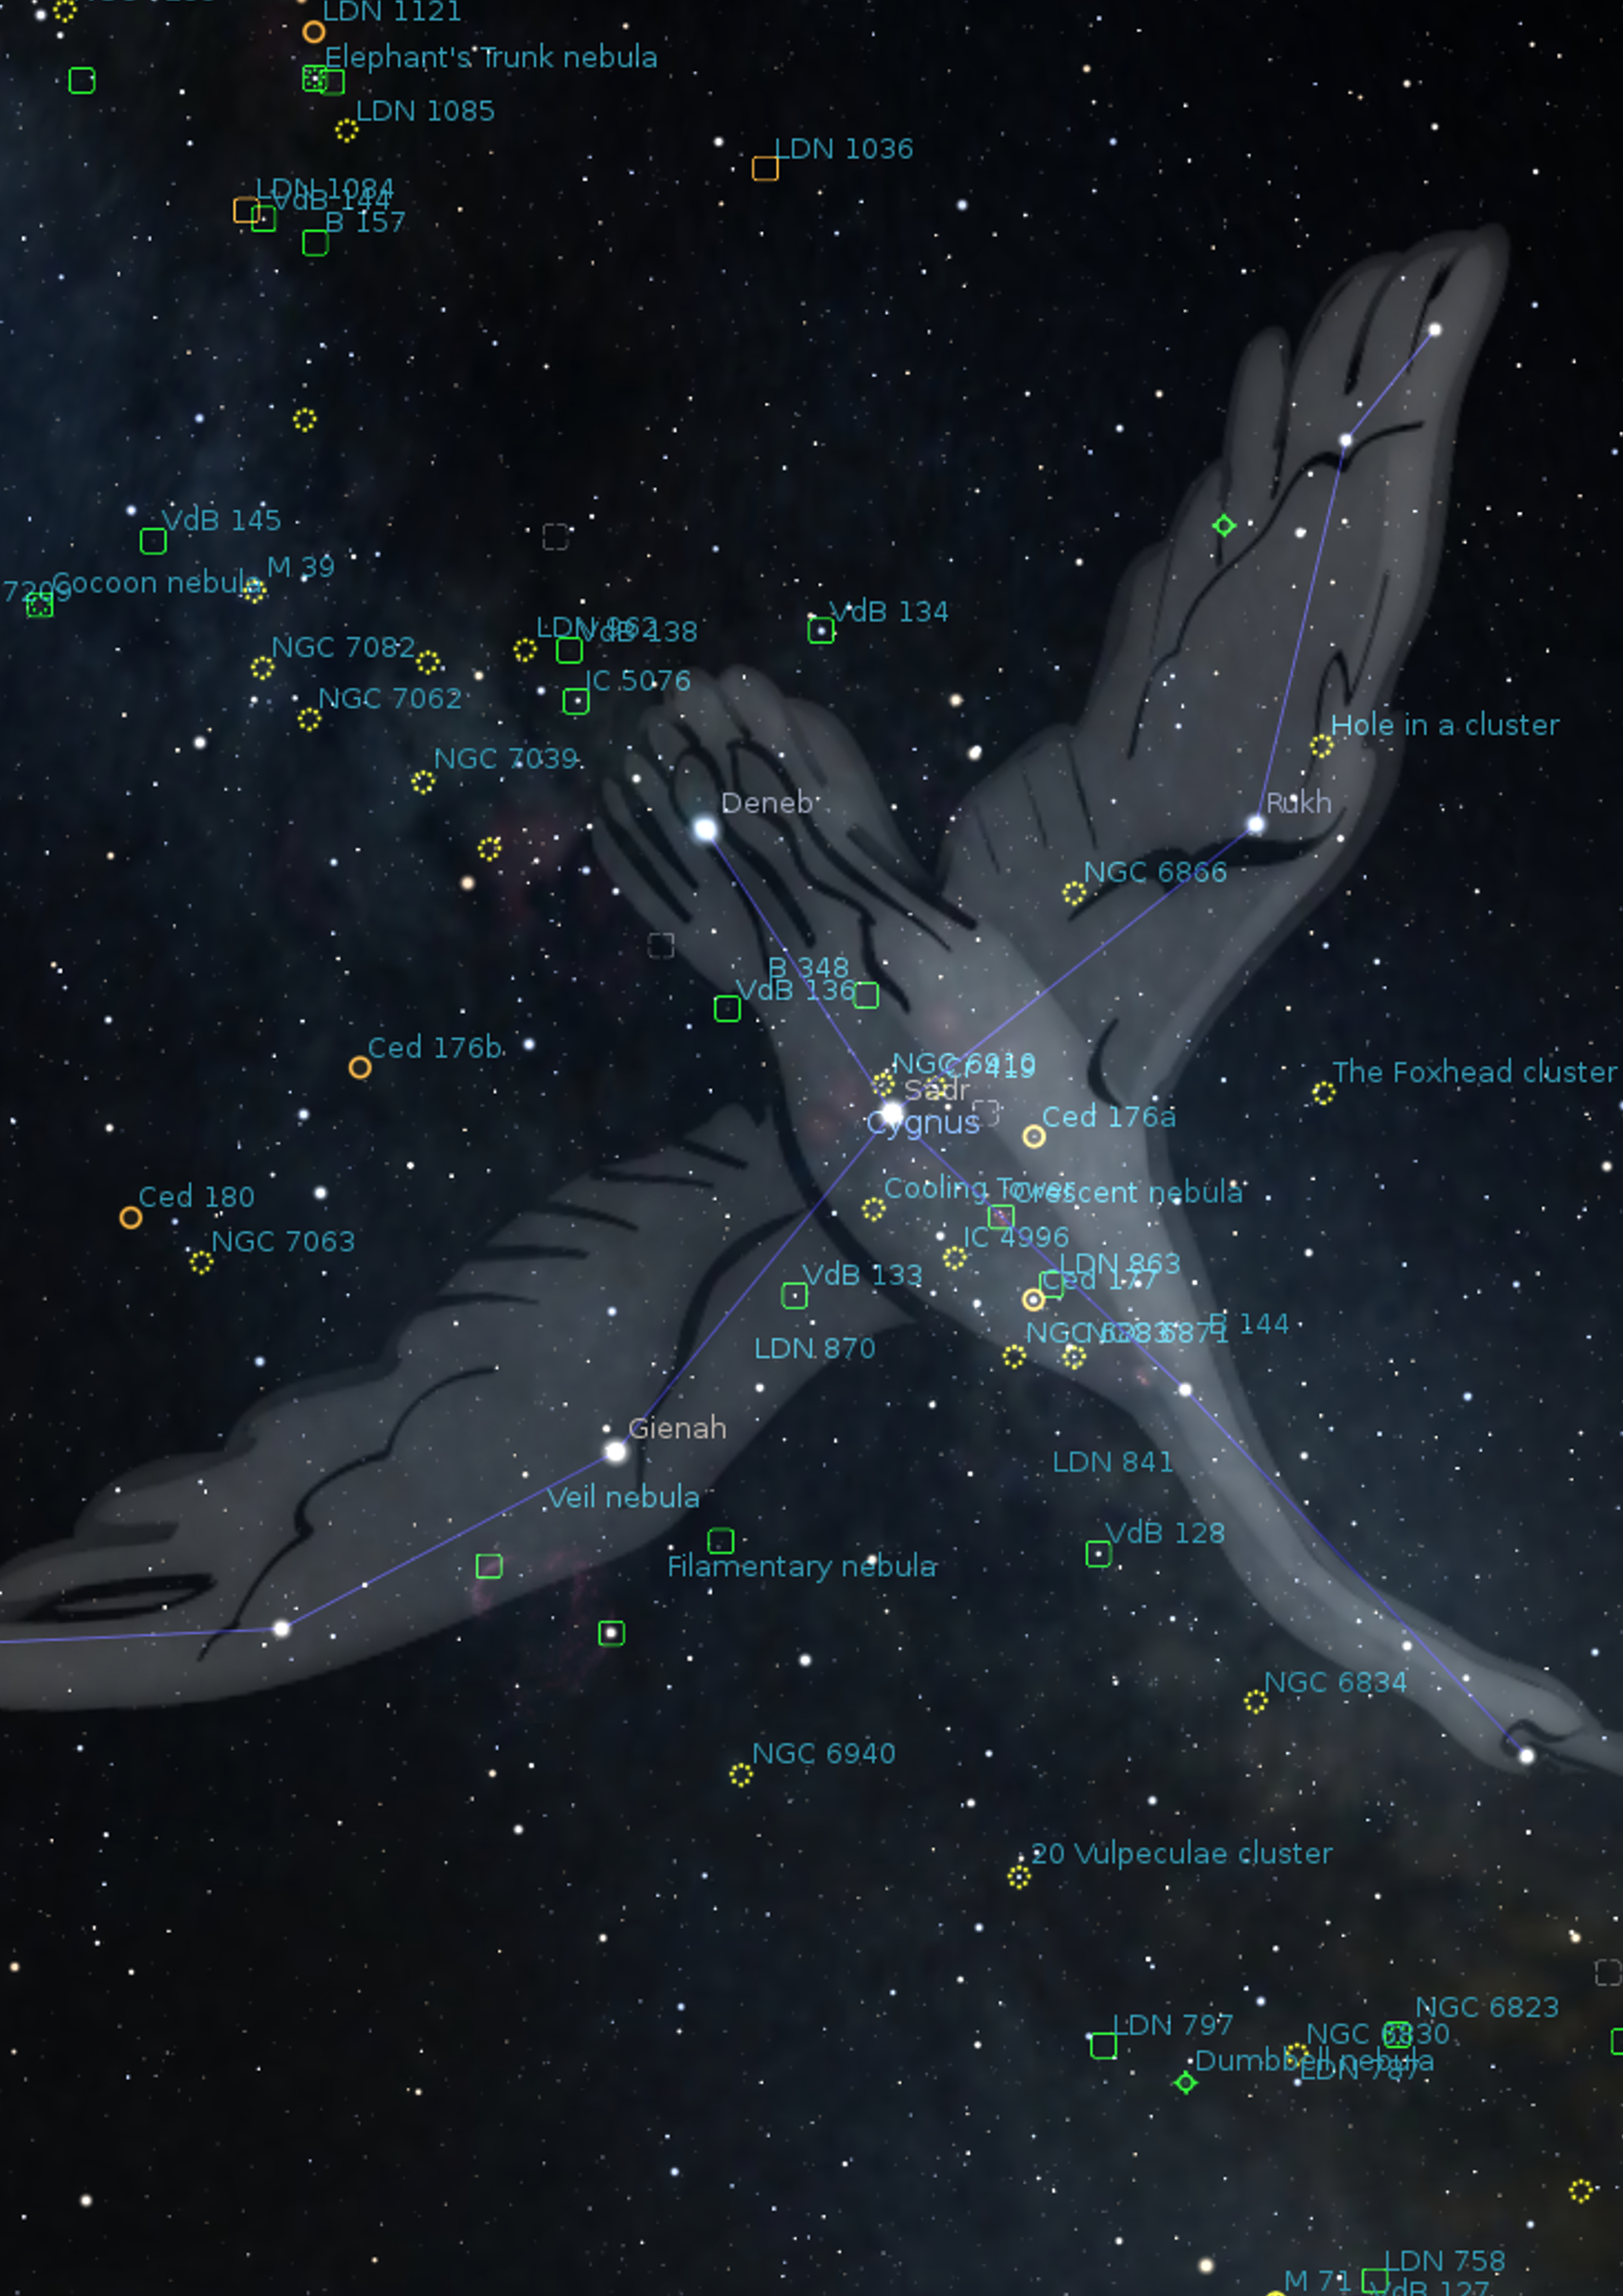
\includegraphics[width=\paperwidth]{bookcover}}; % Background image
\draw[anchor=north] (midpoint) node [fill=ocre!30!white,fill opacity=0.6,text opacity=1,inner sep=1cm]{\Huge\centering\bfseries\sffamily\parbox[c][][t]{\paperwidth}{\centering Stellarium User Guide\\[15pt] % Book title
%{\Large Version 0.15.0-1}\\[20pt] % Subtitle
{\Large Matthew Gates, Barry Gerdes, Alexander Wolf, Georg Zotti}}}; % Author name
\end{tikzpicture}};
\end{tikzpicture}
\vfill
\endgroup

%----------------------------------------------------------------------------------------
%	COPYRIGHT PAGE
%----------------------------------------------------------------------------------------

\newpage
~\vfill
\thispagestyle{empty}

\noindent Copyright \copyright\ 2006-2009 Matthew Gates.\\ % Copyright notice
\noindent Copyright \copyright\ 2013-2014 Barry Gerdes.\\ % Copyright notice
\noindent Copyright \copyright\ 2013-2015 Alexander Wolf.\\ % Copyright notice
\noindent Copyright \copyright\ 2014-2015 Georg Zotti.\\ % Copyright notice

\noindent \textsc{Version 0.15.0-1}\\ % Publisher

\noindent \textsc{stellarium.org}\\ % URL

\noindent Permission is granted to copy, distribute and/or modify this document under the terms of the GNU Free Documentation License, Version 1.2 or any later version published by the Free Software Foundation; with no Invariant Sections, no Front-Cover Texts, and no Back-Cover Texts. A copy of the license is included in the section entitled "GNU Free Documentation License".\\ % License information

\noindent \textit{A first draft, December 2015} % Printing/edition date

%----------------------------------------------------------------------------------------
%	TABLE OF CONTENTS
%----------------------------------------------------------------------------------------

\chapterimage{chapter-bg.png} % Table of contents heading image

\pagestyle{empty} % No headers

\tableofcontents % Print the table of contents itself

\cleardoublepage % Forces the first chapter to start on an odd page so it's on the right

\pagestyle{fancy} % Print headers again

%----------------------------------------------------------------------------------------
%	CHAPTER 1 (Introduction)
%----------------------------------------------------------------------------------------

\chapterimage{chapter-t2-bg} % Chapter heading image

\chapter{Introduction}

\emph{Stellarium} is a software project that allows people to use their
home computer as a virtual planetarium. It calculates the positions of
the Sun and Moon, planets and stars, and draws how the sky would look to
an observer depending on their location and the time. It can also draw
the constellations and simulate astronomical phenomena such as meteor
showers, and solar or lunar eclipses.

Stellarium may be used as an educational tool for teaching about the
night sky, as an observational aid for amateur astronomers wishing to
plan a night's observing, or simply as a curiosity (it's fun!). Because
of the high quality of the graphics that Stellarium produces, it is used
in some real planetarium projector products. Some amateur astronomy
groups use it to create sky maps for describing regions of the sky in
articles for newsletters and magazines.

The development of a powerful scripting system has been continuing for a
number of years now and can now be called operational. The use of a
script was recognised as a perfect way of arranging a display of a
sequence of astronomical events from the earliest versions of Stellarium
and a simple system called the Stratoscript was implemented. The
scipting facility is Stellarium's version of a \emph{Presentation}, a
feature that may be used to run an astronomical or other presentation
for instruction or entertainment from within the Stellarium program. The
original Stratoscript was quite limited in what it could do so a new
Stellarium Scripting System has been developed.

Stellarium is under fairly rapid development, and by the time you read
this guide, a newer version may have been released with even more
features that those documented here. Check for updates to Stellarium at
the Stellarium website.

If you have questions and/or comments about this guide, please email the
author. For comments about Stellarium itself, visit the
\href{https://sourceforge.net/p/stellarium/discussion/278769/}{Stellarium
forums}.



%----------------------------------------------------------------------------------------
%	CHAPTER 2 (Installation)
%----------------------------------------------------------------------------------------

\chapterimage{chapter-bg.png} % Chapter heading image

\chapter{Installation}\label{installation}

\section{System Requirements}\label{system-requirements}

\subsection{Minimum}
\begin{itemize}
\item Linux/Unix; Windows 7 and above\footnote{Since version 0.14.0 only
  classic application can be work on Windows XP. Version 0.12.4 required
  Windows 2000 and above}; OS X 10.7.4 and above\footnote{Version 0.12.4
  required OS X 10.6.8. Version 0.10.6 required OS X 10.5. Version
  0.10.2 runs on OS X 10.3.9}
\item 3D graphics card which supports OpenGL 3.0 and GLSL 1.3\footnote{Version
  0.12.4 required 3D graphics card which supports OpenGL 1.2}
\item 512 MB RAM
\item 250 MB free on disk
\end{itemize}

\subsection{Recommended}
\begin{itemize}
\item Linux/Unix; Windows 7 and above; OS X 10.8.5 and above
\item 3D graphics card which supports OpenGL 3.3 and above\footnote{Version
  0.12.4 required 3D graphics card which supports OpenGL 2.1 and above}
\item 1 GB RAM or more
\item 1.5 GB free on disk
\end{itemize}
 A dark room for realistic rendering --- details like the Milky Way or
star twinkling can't be seen in a bright room.

\section{Downloading}\label{downloading}

Download the correct package for your operating system directly from the
\href{http://stellarium.org}{main page}.

\section{Installation}\label{installation}

\subsection{Windows}\label{windows}

\begin{enumerate}
\item
  Double click on the \texttt{stellarium-0.14.1-win32.exe} (or
  \texttt{stellarium-0.14.1-win64.exe} on Windows x64) file to run the
  installer\footnote{Or \texttt{stellarium-0.14.1-classic-win32.exe} on
    Windows XP.}.
\item
  Follow the on-screen instructions.
\end{enumerate}

\subsection{MacOS X}\label{macos-x}

\begin{enumerate}
\item
  Locate the Stellarium-0.14.1.dmg\footnote{Or
    \texttt{Stellarium-0.10.6-PPC.dmg} for PowerPC MacOS X} file in
  Finder and double click on it or open it using the Disk Utility
  application. Now, a new disk appears on your desktop and Stellarium is
  in it.
\item
  Open the new disk and please take a moment to read the ReadMe file.
  Then drag Stellarium to the Applications folder.
\item
  Note: You should copy Stellarium to the Applications folder before
  running it --- some users have reported problems running it directly
  from the disk image (.dmg).
\end{enumerate}

\subsection{Linux}\label{linux}

Check if your distribution has a package for Stellarium already --- if
so you're probably best off using it. If not, you can download and build
the source.

For ubuntu we provide a package repository with the latest stable
releases. Open a terminal and type:

\texttt{sudo~add-apt-repository~ppa:stellarium/stellarium-releases}\\
\texttt{sudo~apt-get~update}\\
\texttt{sudo~apt-get~install~stellarium}

\section{Running Stellarium}\label{running-stellarium}

\begin{itemize}
\item
  \textbf{Windows} The Stellarium installer creates an item in the
  \textbf{Start Menu} under in \textbf{Programs} section. Select this to
  run \emph{Stellarium}.
\item
  \textbf{MacOS X} Double click on the \emph{Stellarium} application.
  Add it to your \textbf{Dock} for quick access.
\item
  \textbf{Linux} If your distribution had a package you'll probably
  already have an item in the GNOME or KDE application menus. If not,
  just use a open a terminal and type \texttt{stellarium}.
\end{itemize}

%----------------------------------------------------------------------------------------
%	CHAPTER 3 (Interface Guide)
%----------------------------------------------------------------------------------------

\chapterimage{chapter-bg.png} % Chapter heading image

\chapter{Interface Guide}

The way stellarium is shown on the screen is primarily governed by the
menus. These are accessed by dragging the mouse to the left or bottom
edge of the screen

\section{Tour}\label{tour}

\begin{figure}[h]
\centering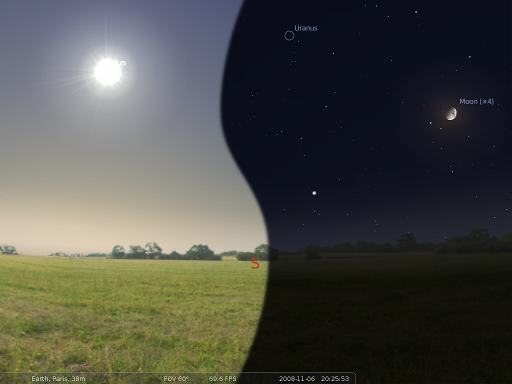
\includegraphics{001}
%\caption{Figure caption}
\end{figure}

At the bottom left of the screen, you can see the status bar. This shows
the current observer location, field of view (FOV), graphics performance
in frames per second (FPS) and the current simulation date and time.

The rest of the view is devoted to rendering a realistic scene including
a panoramic langscape and the sky. If the simulation time and observer
location are such that it is night time, you will see stars, planets and
the moon in the sky, all in the correct positions.

You can drag with the mouse on the sky to look around or use the cursor
keys. You can zoom with the mouse wheel or the page up/page down keys.

If you move the mouse over the status bar, it will move up to reveal a
tool bar which gives quick control over the program.

\subsection{Time Travel}\label{time-travel}

When Stellarium starts up, it sets its clock to the same time and date
as the system clock. However, Stellarium's clock is not fixed to same
time and date as the system clock, or indeed to the same speed. We may
tell Stellarium to change how fast time should pass, and even make time
go backwards! So the first thing we shall do is to travel into the
future! Let's take a look at the time control buttons on the right hand
ride of the tool-bar. If you hover the mouse cursor over the buttons, a
short description of the button's purpose and keyboard shortcut will
appear.

\begin{table}[h]
\centering
\begin{tabular}{l l l}
\toprule
\textbf{Button} & \textbf{Shortcut key} & \textbf{Description}\\
\midrule

\includegraphics[scale=0.75]{timerate_decrease} & J & Decrease the rate at which time passes \\

\includegraphics[scale=0.75]{timerate_normal} & K & Make time pass as normal \\

\includegraphics[scale=0.75]{timerate_increase} & L & Increase the rate at which time passes \\

\includegraphics[scale=0.75]{time_normal} & 8 & Return to the current time \& date \\
\bottomrule
\end{tabular}
\caption{Time Travel}
\end{table}

OK, so lets go see the future! Click the mouse once on the increase time
speed button

\includegraphics[scale=0.5]{timerate_increase}
. Not a whole lot seems to happen. However, take a look at the clock in
the status bar. You should see the time going by faster than a normal
clock! Click the button a second time. Now the time is going by faster
than before. If it's night time, you might also notice that the stars
have started to move slightly across the sky. If it's daytime you might
be able to see the sun moving (but it's less apparent than the movement
of the stars). Increase the rate at which time passes again by clicking
on the button a third time. Now time is really flying!

Let time move on at this fast speed for a little while. Notice how the
stars move across the sky. If you wait a little while, you'll see the
Sun rising and setting. It's a bit like a time-lapse movie. Stellarium
not only allows for moving forward through time - you can go backwards
too!

Click on the real time speed button

\includegraphics[scale=0.5]{timerate_normal} .
The stars and/or the Sun should stop scooting across the sky. Now press
the decrease time speed button

\includegraphics[scale=0.5]{timerate_decrease}
once. Look at the clock. Time has stopped. Click the Decrease time speed
button four or five more times. Now we're falling back through time at
quite a rate (about one day every ten seconds!).

Enough time travel for now. Wait until it's night time, and then click
the Real time speed button. With a little luck you will now be looking
at the night sky.

\subsection{Moving Around the Sky}\label{moving-around-the-sky}

\begin{table}[h]
\centering
\begin{tabular}{l l}
\toprule
\textbf{Key} & \textbf{Description}\\
\midrule
Cursor keys & Pan the view left, right, up and down \\
Page up / Page down & Zoom in and out \\
Backslash (\textbackslash{}) & Auto-zoom out to original field of
view \\
Left mouse button & Select an object in the sky \\
Right mouse button & Clear selected object \\
Mouse wheel & Zoom in and out \\ 
Space & Centre view on selected object \\
Forward-slash (/) & Auto-zoom in to selected object \\
\bottomrule
\end{tabular}
\caption{Moving Around the Sky}
\end{table}

As well as travelling through time, Stellarium lets to look around the
sky freely, and zoom in and out. There are several ways to accomplish
this listed in table above.

Let's try it. Use the cursors to move around left, right, up and down.
Zoom in a little using the Page Up key, and back out again using the
Page Down. Press the backslash key and see how Stellarium returns to the
original field of view (how ``zoomed in'' the view is), and direction of
view.

It's also possible to move around using the mouse. If you left-click and
drag somewhere on the sky, you can pull the view around.

Another method of moving is to select some object in the sky (left-click
on the object), and press the Space key to centre the view on that
object. Similarly, selecting an object and pressing the forward-slash
key will centre on the object and zoom right in on it.

The forward-slash and backslash keys auto-zoom in an out to different
levels depending on what is selected. If the object selected is a planet
or moon in a \emph{sub-system} with a lot of moons (e.g. Jupiter), the
initial zoom in will go to an intermediate level where the whole
sub-system should be visible. A second zoom will go to the full zoom
level on the selected object. Similarly, if you are fully zoomed in on a
moon of Jupiter, the first auto-zoom out will go to the sub-system zoom
level. Subsequent auto-zoom out will fully zoom out and return the
initial direction of view. For objects that are not part of a
sub-system, the initial auto-zoom in will zoom right in on the selected
object (the exact field of view depending on the size/type of the
selected object), and the initial auto-zoom out will return to the
initial FOV and direction of view.

\subsection{Main Tool-bar}\label{main-tool-bar}

\begin{figure}[h]
\centering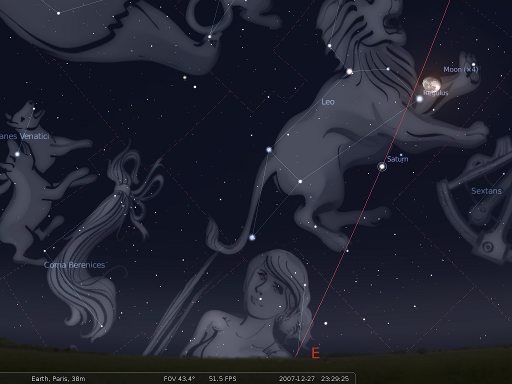
\includegraphics{002}
%\caption{Figure caption}
\end{figure}

Stellarium can do a whole lot more than just draw the stars. Figure
above shows some of Stellarium's visual effects including constellation
line and boundary drawing, constellation art, planet hints, and
atmospheric fogging around the bright Moon. The controls main tool-bar
provides a mechanism for turning on and off the visual effects.

When the mouse if moved to the bottom left of the screen, a second
tool-bar becomes visible. All the buttons in this side tool-bar open and
close dialog boxes which contain controls for further configuration of
the program.

Table below describes the operations of buttons on the main tool-bar and
the side tool-bar, and gives their keyboard shortcuts.

\begin{table}[h]
\centering
\begin{tabular}{l l l l}
\toprule
\textbf{Feature} & \textbf{Button} & \textbf{Key} & \textbf{Description}\\
\midrule
Constellations & 
\includegraphics[scale=0.75]{constellation_button} & C & Draws the constellation lines \\
Constellation Names & 
\includegraphics[scale=0.75]{constellation_name_button}
& V & Draws the name of the constellations \\
Constellation Art & 
\includegraphics[scale=0.75]{constellation_art_button}
& R & Superimposes artistic representations of the constellations over
the stars \\
Equatorial Grid & 
\includegraphics[scale=0.75]{eq_grid_button} & E &
Draws grid lines for the RA/Dec coordinate system \\
Azimuth Grid & 
\includegraphics[scale=0.75]{az_grid_button} & Z &
Draws grid lines for the Alt/Azi coordinate system \\
Toggle Ground & 
\includegraphics[scale=0.75]{ground_button} & G &
Toggles drawing of the ground. Turn this off to see objects that are
below the horizon \\
Toggle Cardinal Points & 
\includegraphics[scale=0.75]{cardinal_button} & Q &
Toggles marking of the North, South, East and West points on the
horizon \\
Toggle Atmosphere & 
\includegraphics[scale=0.75]{atmosphere_button} & A
& Toggles atmospheric effects. Most notably makes the stars visible in
the daytime \\
Deep-Sky Objects & 
\includegraphics[scale=0.75]{nebulae_button} & D &
Toggles marking the positions of Deep-Sky Objects when the FOV is
too wide to see them \\
Planet Hints & 
\includegraphics[scale=0.75]{planets_button} & P &
Toggles indicators to show the position of planets \\
Coordinate System & 
\includegraphics[scale=0.75]{coord_type_button} &
Enter & Toggles between Alt/Azi \& RA/Dec coordinate systems \\
Goto & 
\includegraphics[scale=0.75]{goto_button} &
Space & Centres the view on the selected object \\
Night Mode & 
\includegraphics[scale=0.75]{night_mode_button} &
Ctrl+N & Toggle ``night mode'', which changes the coloring of same
display elements to be easier on the dark-adapted eye. \\
Nebula background images & 
\includegraphics[scale=0.75]{DSS_button} &
{[}none{]} & Toggle ``nebula background images'', which turns the
Textures on or off. \\
Full Screen Mode & 
\includegraphics[scale=0.75]{fullscreen_button} &
F11 & Toggle full screen mode. \\
Flip image (horizontal) & 
\includegraphics[scale=0.75]{fliph_button} &
Ctrl+Shift+H & Flips the image in the horizontal plane. Note this button
is not enable by default. See section {[}sec:imageflipping{]} \\
Flip image (vertical) & 
\includegraphics[scale=0.75]{flipv_button} &
Ctrl+Shift+V & Flips the image in the vertical plane. Note this button
is not enable by default. See section {[}sec:imageflipping{]} \\
Quit Stellarium & 
\includegraphics[scale=0.75]{quit_button} & Ctrl-Q
& Close Stellarium. Note: the keyboard shortcut is COMMAND-Q on OSX
machines \\
Help Window & 
\includegraphics[scale=0.5]{help_button} & F1 &
Show the help window, which lists key bindings and other useful
information \\
Configuration Window & 
\includegraphics[scale=0.5]{config_button} & F2 &
Show the display of the configuration window \\
Search Window & 
\includegraphics[scale=0.5]{find_button} & F3 or
Ctrl+F & Show the display of the object search window \\
View Window & 
\includegraphics[scale=0.5]{view_button} & F4 &
Show the view window \\
Time Window & 
\includegraphics[scale=0.5]{time_button} & F5 &
Show the display of the help window \\
Location Window & 
\includegraphics[scale=0.5]{location_button} & F6
& Show the observer location window (map) \\
\bottomrule
\end{tabular}
\caption{Moving Around the Sky}
\end{table}

\subsection{The Object Search Window}\label{the-object-search-window}

\begin{figure}[h]
\centering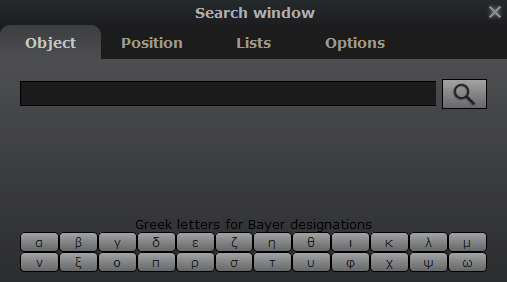
\includegraphics{search_dialog}
\caption{The Object Search Window}
\end{figure}

The Object Search window provides a convenient way to locate objects in
the sky. Simply type in the name of an object to find, and then click
the ``go'' button or press return. Stellarium will point you at that
object in the sky.

As you type, Stellarium will make a list of objects which begin with
what you have typed so far. The first of the list of matching objects
will be highlighted. If you press the TAB key, the selection will change
to the next item in the list. Hitting the RETURN key will go to the
currently highlighted object and close the search dialog.

For example, suppose we want to locate Mimas (a moon of Saturn). After
typing the first letter of the name, \emph{m}, Stellarium makes a list
of objects whose name begins with M: Mars, Mercury, Mimas, Miranda,
Moon. The first item in this list, Mars, is highlighted. Pressing return
now would go to Mars, but we want Mimas. We can either press TAB twice
to highlight Mimas and then hit RETURN, or we can continue to type the
name until it is the first/only object in the list.

\begin{figure}[h]
\centering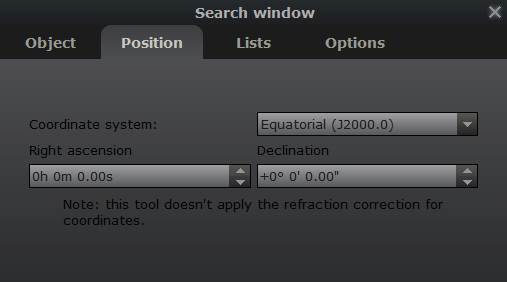
\includegraphics{search_dialog_position}
%\caption{The Object Search Window}
\end{figure}

The Position Search window provides a convenient way to enter a user set
of coordinateslocate objects in the sky. Simply type in the name of an
object to find, and then click the ``go'' button or press return.
Stellarium will point you at that object in the sky.

\begin{figure}[h]
\centering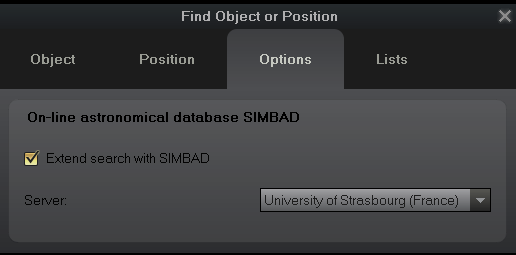
\includegraphics{search_dialog_option}
%\caption{The Object Search Window}
\end{figure}

The Option Search window provides a convenient way to locate objects in
the sky. When the name of an object to find is typed in the object
window and you are connected to the internet and the Extended search is
ticked Stellarium will search the on line SIMBAD data bases for its
coordinates you can and then click the ``go'' button or press return.
Stellarium will point you at that object in the sky even if there is no
object displayed on the screen. The SIMBAD server being used can be
selected from the scroll window

\begin{figure}[h]
\centering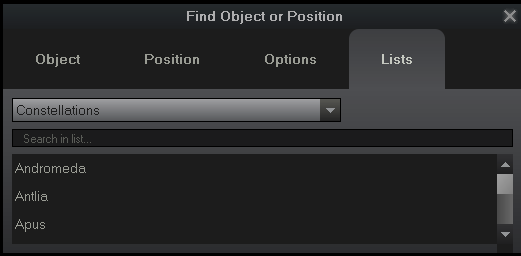
\includegraphics{search_dialog_list}
%\caption{The Object Search Window}
\end{figure}

The List Search window provides a convenient way to locate particular
types of objects in the sky. At the moment the number of choices is
governed by the loaded plug ins. Simply scroll down the first window to
select the type. The name of an object can then be selected from the
list. Press enter and stelarium will go to that object.

\subsection{Help Window}\label{help-window}

\begin{figure}[h]
\centering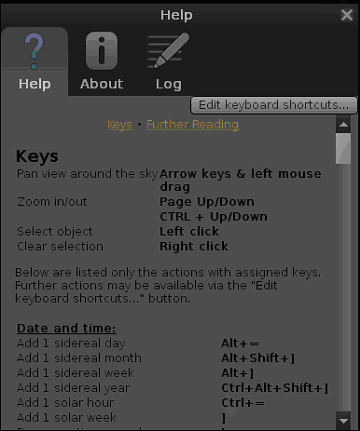
\includegraphics{help_dialog}
\caption{Help Window}
\end{figure}

The Help window lists all Stellarium's key-strokes. Not that some
features are only available as key strokes, so it's a good idea to have
a browse of the information in this window.

\begin{figure}[h]
\centering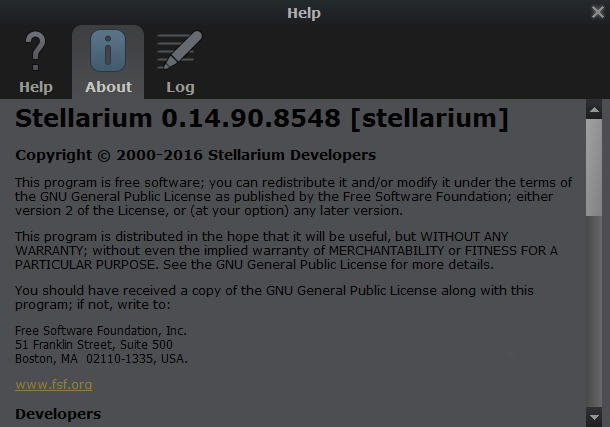
\includegraphics{help_dialog_about}
%\caption{Help Window}
\end{figure}

The About tab in this window will show licensing information, and a list
of people who helped to produce the program.

\begin{figure}[h]
\centering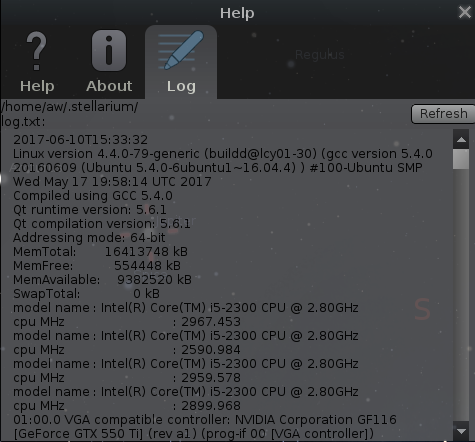
\includegraphics{help_dialog_log}
%\caption{Help Window}
\end{figure}

The help window log lists the loading instructions carried out when
stellarium runs. It is useful to locate the files that stellarium writes
to you computer. It is the master of the copy ``log.txt'' that you will
find in your user area.



%----------------------------------------------------------------------------------------
%	CHAPTER 4 (Configuration)
%----------------------------------------------------------------------------------------

\chapterimage{chapter-bg.png} % Chapter heading image

\chapter{Configuration}

Most of Stellarium's configuration is done using the configuration
window and the view window. To open the configuration window, click the
button on the left side toolbar or press F2. To open the view window
click the button on the left side toolbar or press F4.

Some options may only be configured by editing the configuration file.
See \href{Advanced_Use\#The_Main_Configuration_File}{ configuration
file} for more details.

\section{Setting the Date and Time}\label{setting-the-date-and-time}

\begin{figure}[h]
\centering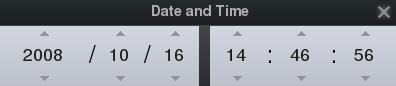
\includegraphics{date_and_time_dialog}
%\caption{Figure caption}
\end{figure}

In addition to the time rate control buttons on the main toolbar, you
can use the date and time window to set the simulation time. The values
for year, month, day, hour, minutes and seconds may be modified by
typing new values, by clicking the up and down arrows above and below
the values, and by using the mouse wheel.

\section{Setting Your Location}\label{setting-your-location}

\begin{figure}[h]
\centering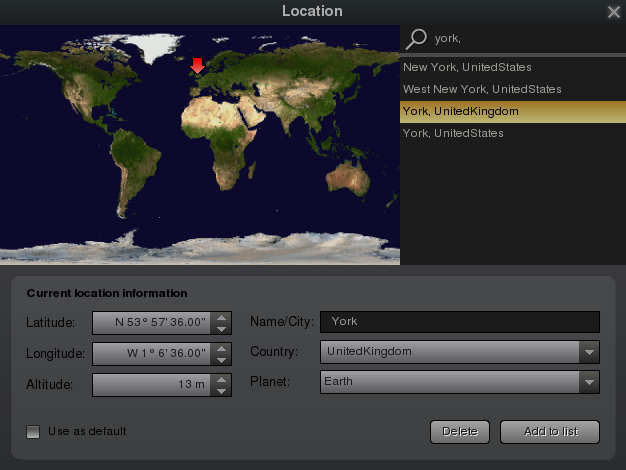
\includegraphics[scale=0.68]{location_dialog}
%\caption{Figure caption}
\end{figure}

The positions of the stars in the sky is dependent on your location on
Earth (or other planet) as well as the time and date. For Stellarium to
show accurately what is (or will be/was) in the sky, you must tell it
where you are. You only need to do this once - Stellarium can save your
location so you won't need to set it again until you move.

To set your location, press F6 to open the location window. There are a
few ways you can set your location:

\begin{enumerate}
\item
  Just click on the map.
\item
  Search for a city where you live using the search edit box at the top
  right of the window, and select the right city from the list.
\item
  Enter a new location using the longitude, latitude and other data.
\end{enumerate}

Once you're happy that the location is set correctly, click on the ``use
as default'' checkbox, and close the location window.

\subsection{The Configuration Window}\label{the-configuration-window}

The configuration window contains general program settings, and many
other settings which do not concern specific display options.

\begin{figure}[h]
\centering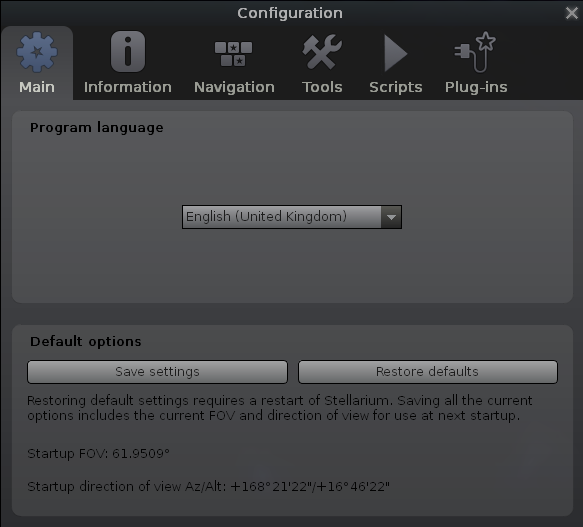
\includegraphics[scale=0.68]{config_dialog_main_tab}
%\caption{Figure caption}
\end{figure}

The Main tab in the configuration window provides controls for changing
the program language, how much information is shown about selected sky
objects, and provides a button for saving the current program
configuration.

\begin{figure}[h]
\centering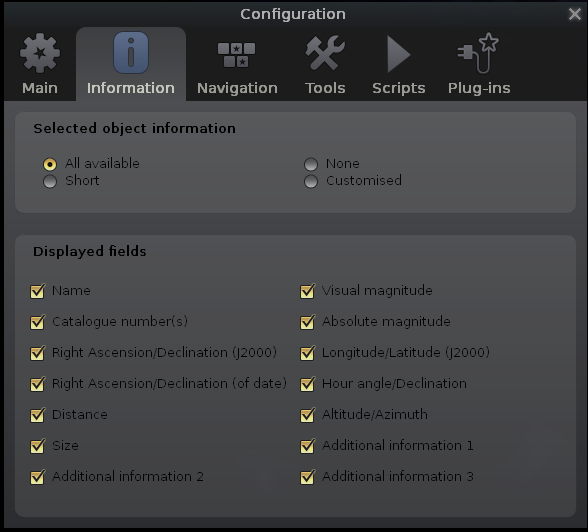
\includegraphics[scale=0.68]{config_dialog_info_tab}
%\caption{Figure caption}
\end{figure}

The Information tab allows you to set the type and amount of information
displayed on a selected object.
\begin{itemize}
\item Ticking or unticking the relevant boxes will control this.
\item The information displays in various colours depending on the type and
level of the stored data
\end{itemize}

\begin{figure}[h]
\centering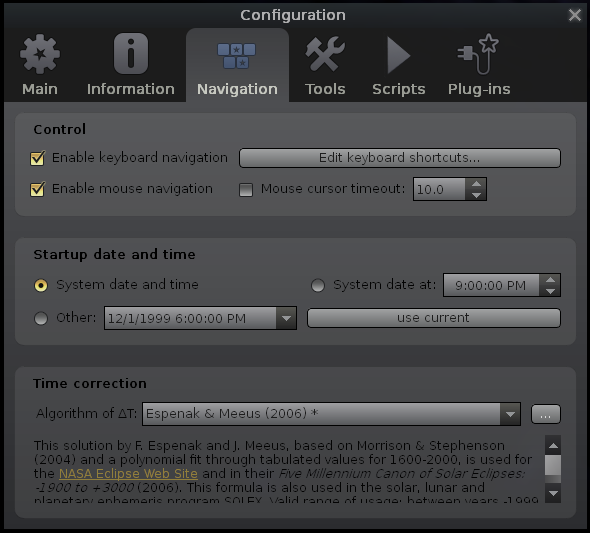
\includegraphics[scale=0.68]{config_dialog_navigation_tab}
%\caption{Figure caption}
\end{figure}

The Navigation tab allows for enabling/disabling of keyboard shortcuts
for panning and zooming the main view, and also how to specify what
simulation time should be used when the program starts:

\begin{itemize}
\item
  When ``Syetem date and time'' is selected, Stellarium will start with
  the simulation time equal to the operating system clock.
\item
  When ``System date at'' is selected, Stellarium will start with the
  same date as the operating system clock, but the time will be fixed at
  the specified value. This is a useful setting for those people who use
  Stellarium during the day to plan observing sessions for the upcoming
  evening.
\item
  When ``Other'' is selected, some fixed time can be chosen which will
  be used every time Stellarium starts.
\end{itemize}

\begin{figure}[h]
\centering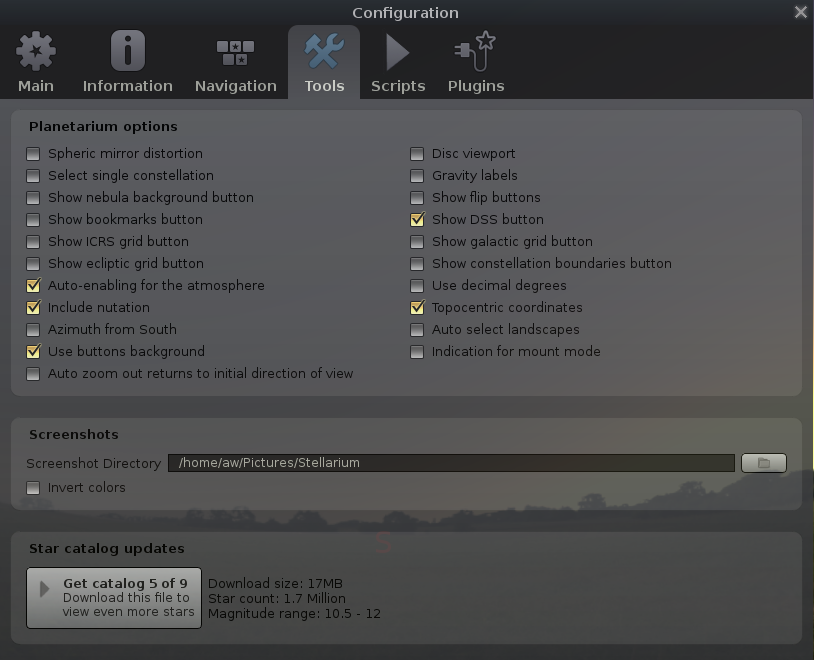
\includegraphics[scale=0.68]{config_dialog_tools_tab}
%\caption{Figure caption}
\end{figure}

The Tools tab of the configuration window contains miscellaneous utility
features:

\begin{itemize}
\item
  \textbf{Show flip buttons} When enabled, two buttons will be added to
  the main tool-bar which allow the main view to be mirrored in the
  vertical and horizontal directions. This is useful when observing
  through telecopes which may cause the image to be mirrored.
\item
  \textbf{Spheric mirror distortion} This option pre-warps the main view
  such that it may be projected onto a spherical mirror using a
  projector. The resulting image will be refected up from the spherical
  mirror in such a way that it may be shone onto a small planetarium
  dome, making a cheap planetarium projection system.
\item
  \textbf{Disc viewport} This option limits masks the main view
  producing the effect of a telescope eyepiece. It is also useful when
  projecting Stellarium's output with a fish-eye lens planetarium
  projector.
\item
  \textbf{Gravity labels} This option makes labels of objects in the
  main view align with the nearest horizon. This means that labels
  projected onto a dome are always alighned properly.
\item
  \textbf{Auto zoom out returns to initial field of view} When enabled,
  this option changes the behaviour of the zoom out key
  (\textbackslash{}) so that it resets the initial direction of view in
  addition to the field of view.
\end{itemize}

\begin{figure}[h]
\centering\includegraphics[scale=0.68]{config_dialog_scripts_tab}
%\caption{Figure caption}
\end{figure}

The Scripts tab allows the selection of pre-assembled scripts bundled
with stellarium that can be run. This list can be expanded in your user
area with your own scripts as required.:

• When a scipt is selected it can be run by pressing the arrow button
and stopped with the stop button. With some scripts the stop button is
inhibited until the script is finished.

• Scripts that use sound will need a version of stellarium compiled at
compile time with sound enabled. It must be pointed out here that sound
when enabled depends on the sound capabilities of you computer plarform
and may not work..

• Scripts that contain Video clips will need a suitable video player
that enabled on tour computer..

\begin{figure}[h]
\centering\includegraphics[scale=0.68]{config_dialog_plugins_tab}
%\caption{Figure caption}
\end{figure}

The Plugins tab. Plug ins need to be enabled at start up to be available
as shown on the bar. This allows for the selection of the plugins that
you wish to be enabled at this time:

\section{The View Settings Window}\label{the-view-settings-window}

The View settings window controls many display features of Stellarium
which are not available via the main toolbar.

\subsection{Sky Tab}\label{sky-tab}

\begin{figure}[h]
\centering\includegraphics[scale=0.68]{view_dialog_sky_tab}
%\caption{Figure caption}
\end{figure}

The Sky tab of the View window{[}fig:viewwinskytab{]} contains settings
for changing the general appearane of the main sky view. Some
hightlights:

\begin{itemize}
\item
  \textbf{Absolute scale} is the size of stars as rendered by
  Stellarium. If you increase this value, all stars will appear larger
  than before.
\item
  \textbf{Relative scale} determines the difference in size of bright
  stars compared to faint stars. Values higher than 1.00 will make the
  brightest stars appear much larger than they do in the sky. This is
  useful for creating star charts, or when learning the basic
  constellations.
\item
  \textbf{Twinkle} controls how much the stars twinkle.
\item
  \textbf{Dynamic eye adaptation} When enabled this feature reduces the
  brightness of faint objects when a bright object is in the field of
  view. This simulates how the eye can be dazzled by a bright object
  such as the moon, making it harder to see faint stars and galaxies.
\item
  \textbf{Light pollution} In urban and suburban areas, the sky is
  brightned by terrestrial light pollution reflected in the atmophere.
  Stellarium simulates light pollution and is calibrated to the
  \emph{Bortle Dark Sky Scale} where 1 means a good dark sky, and 9 is a
  very badly light-polluted sky. See
  \href{Advanced_Use\#Light_Pollution}{Light Pollution} for more
  information.
\item
  \textbf{Planets and satellites} this group of options lets you turn on
  and off various features related to the planets. Simulation of light
  speed will give more precise positions for planetary bodies which move
  rapidly against backround stars (e.g. the moons of Jupiter). The
  \emph{Scale Moon} option will increase the apparent size of the moon
  in the sky, which can be nice for wide field of view shots.
\item
  \textbf{Labels and markers} you can independantly change the amount of
  labels displayed for planets, stars and nebuulae. The further to the
  right the sliders are set, the more labels you will see. Note that
  more labels will also appear as you zoom in.
\item
  \textbf{Shooting stars} Stellarium has a simple meteor simulation
  option. This setting controls how many shooting stars will be shown.
  Note that shooting stars are only visible when the time rate is 1, and
  might not be visiable at some times of day. Meteor showers are not
  currently simulated.
\end{itemize}

\subsection{Marking Tab}\label{marking-tab}

\begin{figure}[h]
\centering\includegraphics[scale=0.68]{view_dialog_markings_tab}
%\caption{Figure caption}
\end{figure}

The Markings tab of the View window controls the following features:

\begin{itemize}
\item
  \textbf{Celestial sphere} this group of options makes it possible to
  plot various grids and lines in the main view.
\item
  \textbf{Constellations} these controls let you turn on and off
  constellation lines, names, art and boundaries, and control the
  brightness of the constellation artwork.
\item
  \textbf{Projection} Selecting items in this list changes the
  projection method which Stellarium uses to draw the sky. Options are:

  \begin{itemize}
  \item
    \textbf{cylinder} The full name of this projection mode is
    \emph{cylindrical equidistant projection}. The maximum field of view
    in this mode is 233\degree.
  \item
    \textbf{equal area} The full name of this projection method is,
    \emph{Lambert azimuthal equal-area projection}. The maximum field of
    view is 360\degree.
  \item
    \textbf{fish-eye} Stellarium draws the sky using \emph{azimuthal
    equidistant projection}. In fish-eye projection, straight lines
    become curves when they appear a large angular distance from the
    centre of the field of view (like the distortions seen with very
    wide angle camera lenses). This is more pronounced as the user zooms
    out. The maximum field of view in this mode is 180\degree.
  \item
    \textbf{Hammer-Aitoff} The Hammer projection is an equal-area map
    projection, described by Ernst Hammer in 1892 and directly inspired
    by the Aitoff projection. The maximum field of view in this mode is
    360\degree.
  \item
    \textbf{mercator} Mercator projection preserves the angles between
    objects, and the scale around an object the same in all directions.
    The maximum field of view in this mode is 233\degree.
  \item
    \textbf{orthographic} Orthographic projection is related to
    perspective projection, but the \emph{point of perspective} is set
    to an infinite distance. The maximum field of view is 180\degree.
  \item
    \textbf{perspective} Perspective projection keeps the horizon a
    straight line. The maximum field of view is 150\degree. The mathematical
    name for this projection method is \emph{gnomonic projection}.
  \item
    \textbf{stereographic} This mode is similar to fish-eye projection
    mode. The maximum field of view in this mode is 235\degree.
  \end{itemize}
\end{itemize}

\subsection{Landscape Tab}\label{landscape-tab}

\begin{figure}[h]
\centering\includegraphics[scale=0.68]{view_dialog_landscape_tab}
%\caption{Figure caption}
\end{figure}

The Landscape tab of the View window controls the landscape graphics
(ground). To change the landscape graphics, select a landscape from the
list on the left side of the window. A description of the landscape will
be shown on the right.

Note that while landscape can include information about where the
landscape graphics were taken (planet, longitude, latitude and
altitude), this location does not have to be the same as the location
selected in the Location window, although you can set up Stellarium such
that selection of a new landscape will alter the location for you.

The controls at the bottom right of the window operate as follows:

\begin{itemize}
\item
  \textbf{Show ground} This turns on and off landscape rendering (same
  as the button in the main tool-bar).
\item
  \textbf{Show\_fog} This turns on and off rendering of a band of
  fog/haze along the horizon.
\item
  \textbf{Use associated planet and position} When enabled, selecting a
  new landscape will automatically update the observer location.
\item
  \textbf{Use this landscape as default} Selecting this option will save
  the landscape into the program configuration file so that the current
  landscape will be the one used when Stellarium starts.
\end{itemize}

\subsubsection{Starlore Tab}\label{starlore-tab}

\begin{figure}[h]
\centering\includegraphics[scale=0.68]{view_dialog_starlore_tab}
%\caption{Figure caption}
\end{figure}

The Starlore tab of the View window controls what culture's
constellations and bright star names will be used in the main display.
Some cultures have constellation art (Western and Inuit), and the rest
do not.



%----------------------------------------------------------------------------------------
%	CHAPTER X (Astronomical Concepts)
%----------------------------------------------------------------------------------------

%% Status:
%% AW 2015-12-27 from wiki or old sources?
%% GZ 2016-01-11 Some first amendments and additions, figure captions, references, index entries.
%% TODO: update all references and citations. 
%% TODO: Update the extra lines which can now be displayed in Stellarium. (Meridian, horizon, colures, ...) 

\chapter{Astronomical Concepts}
\label{ch:Concepts}

This section includes some general notes on astronomy in an effort to
outline some concepts that are helpful to understand features of
Stellarium. Material here is only an overview, and the reader is
encouraged to get hold of a couple of good books on the subject. A good
place to start is a compact guide and ephemeris such as the
\emph{National Audubon Society Field Guide to the Night Sky}\footnote{\url{http://www.amazon.com/National-Audubon-Society-Field-Series/dp/0679408525}}. Also recommended is a
more complete textbook such as \emph{Universe}. %%{[}universe{]}. %% REF MISSING?
There are also some nice resources on the net, like the
\emph{Wikibooks Astronomy book}\footnote{\url{http://en.wikibooks.org/wiki/Subject:Astronomy}}.

\section{The Celestial Sphere}
\label{sec:Concepts:CelestialSphere}

The \indexterm{Celestial Sphere} is a concept which helps us think about the
positions of objects in the sky. Looking up at the sky, you might
imagine that it is a huge dome or top half of a sphere, and the stars
are points of light on that sphere. Visualising the sky in such a
manner, it appears that the sphere moves, taking all the stars with it
--- it seems to rotate. Watching the movement of the stars we can see
that they seem to rotate around a static point about once a day.
Stellarium is the perfect tool to demonstrate this!

\begin{enumerate}
\item Open the location dialog (\key{F6}). Set the location to be
  somewhere in mid-Northern latitudes. (Just click on the map to
  select a location, or fine-tune with the settings.) The United
  Kingdom is an ideal location for this demonstration.
\item Turn off atmospheric rendering \key{A} and ensure cardinal points are
  turned on (\key{Q}). This will keep the sky dark so the Sun doesn't prevent us
  from seeing the motion of the stars when it is above the horizon.
\item Pan round to point North, and make sure the field of view is
  about $90\degree$.
\item Pan up so the `N' cardinal point on the horizon is at the bottom
  of the screen.
\item Now increase the time rate. Press \key{K}, \key{L}, \key{L},
  \key{L}, \key{L} -- this should set the time rate so the stars can
  be seen to rotate around a point in the sky about once every ten
  seconds. If you watch Stellarium's clock you'll see this is the time
  it takes for one day to pass at this accelerated rate.
\end{enumerate}

The point which the stars appear to move around is one of the
\indexterm{Celestial Poles}.

The apparent movement of the stars is due to the rotation of the Earth.
Our location as the observer on the surface of the Earth affects how we
perceive the motion of the stars. To an observer standing at Earth's
North Pole, the stars all seem to rotate around the \indexterm{zenith} (the
point directly upward). As the observer moves South towards the equator,
the location of the celestial pole moves down towards the horizon. At
the Earth's equator, the North celestial pole appears to be on the
Northern horizon.

Similarly, observers in the Southern hemisphere see the Southern
celestial pole at the zenith when they are at the South pole, and it
moves to the horizon as the observer travels towards the equator.

\begin{enumerate}
\item
  Leave time moving on nice and fast, and open the configuration window.
  Go to the location tab and click on the map right at the top -- i.e.,
  set your location to the North pole. See how the stars rotate parallel to the horizon, around a
  point right at the top of the screen. With the field of view set to
  $90\degree$ and the horizon at the bottom of the screen, the top of the screen
  is the zenith.
\item
  Now click on the map again, this time a little further South. You
  should see the positions of the stars jump, and the centre of rotation
  has moved a little further down the screen.
\item
  Click on the map even further towards and equator. You should see the
  centre of rotation having moved down again.
\end{enumerate}

To help with the visualisation of the celestial sphere, turn on the
equatorial grid by clicking the button on the main tool-bar or pressing
the \key{E} key. Now you can see grid lines drawn on the sky. These
lines are like lines of longitude and latitude on the Earth, but drawn
for the celestial sphere.

The \indexterm{Celestial Equator} is the line around the celestial sphere
that is half way between the celestial poles -- just as the Earth's
equator is the line half way between the Earth's poles.




\section{Coordinate Systems}
\label{sec:Concepts:CoordinateSystems}

\subsection{Altitude/Azimuth Coordinates}
\label{sec:Concepts:AltAz}

\begin{figure}[h]
\centering\includegraphics[scale=1.8]{cs_azi}
\caption{Altitude/Azimuth (Horizontal) Coordinate System}
\label{fig:AltAz}
\end{figure}

The \indexterm{Altitude/Azimuth} coordinate system (also called
\indexterm{Horizontal Coordinate System})can be used to describe a
direction of view (the \indexterm{azimuth} angle) and an angular
height in the sky (the \indexterm{altitude} angle). The azimuth angle
is measured clockwise round from due North\footnote{In some textbooks
  azimuth is counted from south. There is no global authority to
  decide upon this issue, just be aware of this when you compare
  numbers with other sources.}. Hence North itself is 0$\degree$, East
$90\degree$, Southwest is $225\degree$ and so on.  The altitude angle
is measured up from the \indexterm{mathematical horizon}, which is
just halfway between ``straight up'' and ``straight down'', without
regard to the landscape. Looking directly up (at the
\indexterm{zenith}) would be $90\degree$, half way between the zenith
and the horizon is $45\degree$ and so on. The point opposite the
zenith is called the \indexterm{nadir}.

The Altitude/Azimuth coordinate system is attractive in that it is
intuitive -- most people are familiar with azimuth angles from bearings
in the context of navigation, and the altitude angle is something most
people can visualise pretty easily.

However, the altitude/azimuth coordinate system is not suitable for
describing the general position of stars and other objects in the sky --
the altitude and azimuth values for a celestial object change with
time and the location of the observer.

Stellarium can draw grid lines for altitude/azimuth coordinates. Use the
button on the main tool-bar to activate this grid, or press the \key{Z} key.

\subsection{Right Ascension/Declination Coordinates}
\label{sec:Concepts:Equatorial}

\begin{figure}[h]
\centering\includegraphics[scale=1.8]{cs_equ}
\caption{Equatorial Coordinates}
\label{fig:EquatorialCoordinates}
\end{figure}

Like the Altitude/Azimuth system, the \indexterm{Right Ascension/Declination}
(RA/Dec) Coordinate System (or \indexterm{Equatorial Coordinate System}) uses two angles to describe positions in the
sky. These angles are measured from standard points on the celestial
sphere. \indexterm{Right ascension} $\alpha$ and \indexterm{declination} $\delta$ are to the celestial sphere what
longitude and latitude are to terrestrial map makers.

The Northern celestial pole has a declination of $\delta=90\degree$, the celestial
equator has a declination of $\delta=0\degree$, and the Southern celestial pole has a declination of $\delta=-90\degree$.

Right ascension is measured as an angle round from a point in the sky
known as the \indexterm{First Point of Aries}, in the same way that longitude
is measured around the Earth from Greenwich. Figure~\ref{fig:EquatorialCoordinates} illustrates
RA/Dec coordinates.

Unlike Altitude/Azimuth coordinates, RA/Dec coordinates of a star do
not change if the observer changes latitude, and do not change over
the course of the day due to the rotation of the Earth (the story is
complicated a little by precession (section~\ref{sec:Concepts:Precession}) and
parallax (section~\ref{sec:Concepts:Parallax}). RA/Dec coordinates are
frequently used in star catalogues such as the Hipparcos catalogue.

Stellarium can draw grid lines for RA/Dec coordinates. Use the button on
the main tool-bar to activate this grid, or press the \key{E} key.

\section{Units}
\label{sec:Concepts:Units}

\subsection{Distance}
\label{sec:Concepts:Distance}

As \name{Douglas Adams} pointed out in the Hitchhiker's Guide to the
Galaxy{[}hhg{]},

\begin{quote}
  Space is big. You just won't believe how vastly, hugely,
  mind-bogglingly big it is. I mean, you may think it's a long way
  down the road to the chemist's, but that's just peanuts to
  space.{[}hhg{]}
\end{quote}
Astronomers use a variety of units for distance that make sense in the
context of the mind-boggling vastness of space.

\begin{description}
\item[Astronomical Unit (AU)] This is the mean Earth-Sun
  distance. Roughly 150 million kilometres
  ($1.49598 \times 10^8\km$). The AU is used mainly when
  discussing the solar system -- for example the distance of various
  planets from the Sun.
\item[Light year (LY)] A light year is not, as some people believe, a
  measure of time. It is the distance that light travels in a
  year. The speed of light being approximately 300,000 kilometres per
  second means a light year is a very large distance indeed, working
  out at about 9.5 trillion kilometres
  ($9.46073\times10^{12}\km$). Light years are most frequently used
  when describing the distance of stars and galaxies or the sizes of
  large-scale objects like galaxies, nebulae etc.
\item[Parsec (pc)] A parsec is defined as the distance of an object
  that has an annual parallax of 1~second of arc. This equates to
  3.26156 light years ($3.08568\times10^{13}\km$). Parsecs (and derivatives: kiloparsec \kpc, megaparsec \Mpc) are most
  frequently used when describing the distance of stars or the sizes
  of large-scale objects like galaxies, nebulae etc.
\end{description}

\subsection{Time}\label{time}

\begin{figure}[h]
\centering\includegraphics[scale=2.2]{sidereal_day}
\caption{Sidereal day}
\label{fig:SiderealDay}
\end{figure}

The length of a day is defined as the amount of time that it takes for
the Sun to travel from the highest point in the sky at mid-day to the
next high-point on the next day. In astronomy this is called a
\emph{solar day}. The apparent motion of the Sun is caused by the
rotation of the Earth. However, in this time, the Earth not only spins,
it also moves slightly round its orbit. Thus in one solar day the Earth
does not spin exactly $360\degree$ on its axis. Another way to measure day
length is to consider how long it takes for the Earth to rotate exactly
$360\degree$. This is known as one \emph{sidereal day}.

Figure~\ref{fig:SiderealDay} illustrates the motion of the Earth as
seen looking down on the Earth orbiting the Sun. The red triangle on the
Earth represents the location of an observer. The figure shows the Earth
at four times:

\begin{enumerate}
\item
  The Sun is directly overhead - it is mid-day.
\item
  Twelve hours have passed since 1. The Earth has rotated round and the
  observer is on the opposite side of the Earth from the Sun. It is
  mid-night. The Earth has also moved round in its orbit a little.
\item
  The Earth has rotated exactly $360\degree$. Exactly one sidereal day has
  passed since 1.
\item
  It is mid-day again -- exactly one solar day since 1. Note that the
  Earth has rotated more than $360\degree$ since 1.
\end{enumerate}

It should be noted that in figure~\ref{fig:SiderealDay} the sizes of
the Sun and Earth and not to scale. More importantly, the distance the
Earth moves around its orbit is much exaggerated. The Earth takes a
year to travel round the Sun --
$365\frac{1}{4}$ solar days. The length of a
sidereal day is about 23 hours, 56 minutes and 4 seconds.

\subsubsection{Sidereal Time}
\label{sec:Concepts:SiderealTime}

It takes exactly one sidereal day for the celestial sphere to make one
revolution in the sky. Astronomers find \indexterm{sidereal time}
useful when observing. This is the Right Ascension which is currently
passing the meridian line.  When visiting observatories, look out for
doctored alarm clocks that have been set to run in sidereal time!



\subsection{Angles}
\label{sec:Concepts:Angles}

Astronomers typically use degrees to measure angles. Since many
observations require very precise measurement, the degree is subdivided
into sixty \emph{minutes of arc} also known as \emph{arc-minutes}. Each
minute of arc is further subdivided into sixty \emph{seconds of arc}, or
\emph{arc-seconds}. Thus one degree is equal to 3600 seconds of arc.
Finer grades of precision are usually expressed using the SI prefixes
with arc-seconds, e.g. \emph{milli arc-seconds} (one milli arc-second is
one thousandth of an arc-second).

\subsubsection{Notation}

Degrees are denoted using the $\degree$ symbol after a number. Minutes of arc are denoted with a~$'$, and seconds of arc are denoted using~$''$. Angles are frequently given in two formats:

\begin{enumerate}
\item
  DMS format --- degrees, minutes and seconds. For example $90\degree15'12''$.
  When more precision is required, the seconds component may include a
  decimal part, for example $90\degree15'12.432''$.
\item
  Decimal degrees, for example $90.2533\degree$
\end{enumerate}

\subsubsection{Handy Angles}
\label{sec:Concepts:Angles:HandyAngles}
\index{Handy Angles}

Being able to estimate angular distance can be very useful when trying
to find objects from star maps in the sky. One way to do this with a
device called a \indexterm{crossbow}.

%% GZ TODO: Add figure of my crossbow!

Crossbows are a nice way get an idea of angular distances, but carrying
one about is a little cumbersome. A more convenient alternative is to
hold up an object such as a pencil at arm's length. If you know the
length of the pencil, $d$, and the distance of it from your eye, $D$, you
can calculate its angular size, $\theta$ using this formula:

\begin{equation}
\label{eq:handyAngle}
\theta=2 \cdot \arctan{\left(\frac{d}{2 \cdot D}\right) }
\end{equation}


\noindent Another, more handy (ahem!) method is to use the size of your hand at
arm's length:

\begin{description}
\item[Tip of little finger] About 1\degree 
\item[Middle three fingers] About 4\degree 
\item[Across the knuckles of the fist] About 10\degree 
\item[Open hand] About 18\degree
\end{description}

Using you hand in this way is not very precise, but it's close enough
to give you some way to translate an idea like ``Mars will be
$45\degree$ above the Southeastern horizon at 21:30''. Of course,
there is variation from person to person, but the variation is
compensated for somewhat by the fact that people with long arms tend
to have larger hands. In exercise~\ref{sec:Exercises:handyAngles} you
will work out your own ``handy angles''.



\subsection{The Magnitude Scale}
\label{sec:Concepts:Magnitudes}


When astronomers talk about magnitude, they are referring to the
brightness of an object. How bright an object appears to be depends on
how much light it is giving out and how far it is from the observer.
Astronomers separate these factors by using two measures: \indexterm{absolute
magnitude} (Mag or $M$) which is a measure of how much light is being
given out by an object, and \indexterm{apparent magnitude} (mag or $m$) which
is how bright something appears to be in the sky.

For example, consider two 100 watt lamps, one which is a few meters
away, and one which is a kilometre away. Both give out the same amount
of light -- they have the same absolute magnitude. However the nearby
lamp seems much brighter -- it has a much greater apparent magnitude.
When astronomers talk about magnitude without specifying whether they
mean apparent or absolute magnitude, they are usually referring to
apparent magnitude.

The magnitude scale has its roots in antiquity. The Greek astronomer
\name{Hipparchus} defined the brightest stars in the sky to be \emph{first
magnitude}, and the dimmest visible to the naked eye to be \emph{sixth
magnitude}. In the 19th century British astronomer \name{Norman Pogson}
quantified the scale more precisely, defining it as a logarithmic scale
where a magnitude~1 object is 100~times as bright as a magnitude~6
object (a difference of five magnitudes). The zero-point of the modern
scale was originally defined as the brightness of the star Vega, however
this was re-defined more formally in 1982\cite{landolt}. Objects brighter
than Vega are given negative magnitudes.

The absolute magnitude of a star is defined as the magnitude a star
would appear if it were 10 parsecs from the observer.

Table~\ref{tab:Concepts:Magnitudes} lists several objects that may be seen
in the sky, their apparent magnitude and their absolute magnitude where
applicable (only stars have an absolute magnitude value. The planets and
the Moon don't give out light like a star does -- they reflect the light
from the Sun).

\begin{table}[htb]
  \centering
%  \begin{tabular}[t]{lll}
%  \end{tabular}
\begin{longtable}[c]{@{}lll@{}}
\toprule
\emph{Object} & $m$ & $M$\tabularnewline
The Sun & -27 & 4.8\tabularnewline
Vega & 0.05 & 0.6\tabularnewline
Betelgeuse & 0.47 & -7.2\tabularnewline
Sirius (the brightest star) & -1.5 & 1.4\tabularnewline
Venus (at brightest) & -4.4 & ---\tabularnewline
Full Moon (at brightest) & -12.6 & ---\tabularnewline
\bottomrule
\end{longtable}
  \caption{Magnitudes of a few objects}
  \label{tab:Concepts:Magnitudes}
\end{table}


\subsection{Luminosity}
\label{sec:Concepts:Luminosity}

\emph{Luminosity} is an expression of the total energy radiated by a
star. It may be measured in watts, however, astronomers tend to use
another expression --- \emph{solar luminosities} where an object with
twice the Sun's luminosity is considered to have two solar luminosities
and so on. Luminosity is related to absolute magnitude.

\section{Precession}
\label{sec:Concepts:Precession}

\begin{figure}[htb]
\centering\includegraphics[scale=1.4]{obliquity_ecliptic}
\caption{Ecliptic obliquity}
\label{fig:Obliquity}
\end{figure}

As the Earth orbits the Sun throughout the year, the axis of rotation
(the line running through the rotational poles of the Earth) seems
to point towards the same position on the celestial sphere, as can be
seen in figure~\ref{fig:Obliquity}. The angle between the axis
of rotation and the perpendicular of the orbital plane is called the
\indexterm{obliquity of the ecliptic}. It is currently about $23\degree27'$.

\begin{figure}[htb]
\centering\includegraphics[scale=2.0]{precession}
\caption{Precession}
\label{fig:Precession}
\end{figure}


Observed over very long periods of time the direction the axis of
rotation points to does actually change. The angle between the axis of
rotation and the orbital plane stays fairly constant, but the
direction the axis points --- the position of the celestial pole ---
transcribes a circle on the stars in the celestial sphere. The motion
is similar to the way in which a gyroscope slowly twists, as
figure~\ref{fig:Precession} illustrates. This process is called
\indexterm{precession}. The circles can be shown in Stellarium: From
the View menu (\key{F4}), tab ``Markings'', switch on ``Precession
Circles''.

Precession is a slow process. The axis of rotation twists through a
full $360\degree$ about once every 28,000 years. However, over these
long times other gravitational perturbations (``planetary
precession'') play a role, and what may be thought of as rigid
``precession circle'' can actually only show the instantaneous
(current) state. Over millennia the circle slightly varies.

Precession has some important implications:

\begin{enumerate}
\item RA/Dec coordinates change over time, albeit slowly. Measurements
  of the positions of stars recorded using RA/Dec coordinates must
  also include a date (``equinox'') for those coordinates. Therefore
  the current star catalogues list their objects for the epoch and
  equinox J2000.0.
\item
  Polaris, the pole star, won't stay a good indicator of the location of
  the Northern celestial pole. In 14,000 years time Polaris will be
  nearly $47\degree$ away from the celestial pole!
\end{enumerate}


\section{Parallax}
\label{sec:Concepts:Parallax}


Parallax is the change of angular position of two stationary points
relative to each other as seen by an observer, due to the motion of said
observer. Or more simply put, it is the apparent shift of an object
against a background due to a change in observer position.

This can be demonstrated by holding ones thumb up at arm's length.
Closing one eye, note the position of the thumb against the background.
After swapping which eye is open (without moving), the thumb appears to
be in a different position against the background.

\subsection{Geocentric and Topocentric Observations}
\label{sec:Concepts:Topocentric}

%% Author GZ 2016-01-11

When computing planetary positions was done manually by adding numbers
tabulated in yearly almanacs, computing the Earth's position and, say,
position of a minor planet was usually good enough to find the object
in the sky. In both cases, the exact numbers refer to the
gravitational centres of the respective bodies. However, we are
sitting on Earth's surface, so the observed planet will be seen in a
slightly shifted location. The amount for objects in the inner solar
system is usually just a few arcseconds and indeed negligible when we
just want to find an object. But it makes a difference when it comes
to observations of stellar occultations by planets or asteroids. Such
a body may measure only a few tens of kilometres, so the shadow track
which it leaves on Earth's surface is of approximately the same
size.\footnote{Unfortunately Stellarium (as of V0.14) is not accurate
  enough to reliably compute such occultations. Even a deviation of
  0.5 arcseconds is too much here.}

A much closer and bigger object is the Moon, which can also occult
stars. It can even occult the one big star we call the Sun: this is a
Solar Eclipse. And here it makes a huge difference where on the planet
you are located. 

If you are interested in astronomical computing, you may still be
interested in geocentric numerical results. From the Settings panel
(\key{F2}), tab ``Tools'', there is a checkbox for ``Topocentric
Coordinates''. Switch it off to put yourself into the center of the
planet you are located.

\subsection{Stellar Parallax}
\label{sec:Concepts:StellarParallax}

\begin{figure}[tb]
\centering\includegraphics[scale=2.0]{parallax}
\caption{Stellar Parallax}
\label{fig:Parallax}
\end{figure}

A similar thing happens due to the Earth's motion around the Sun. Nearby
stars appear to move against more distant background stars, as
illustrated in figure~\ref{fig:Parallax}.
The movement of nearby stars against the background is called
\emph{stellar parallax}, or \emph{annual parallax}.

Since we know the distance the radius of the Earth's orbit around the
Sun from other methods, we can use simple geometry to calculate the
distance of the nearby star if we measure annual parallax.

As can be seen from figure~\ref{fig:Parallax}, the annual
parallax $p$ is half the angular distance between the apparent positions
of the nearby star. The distance of the nearby object is $d$. Astronomers
use a unit of distance called the parsec ($\pc$) which is defined as the
distance at which a nearby star has $p=1''$.

Even the nearest stars exhibit very small movement due to
parallax. The closest star to the Earth other than the Sun is Proxima
Centauri. It has an annual parallax of $0.77199''$, corresponding to a
distance of $1.295\pc$ (4.22 light years).

Even with the most sensitive instruments for measuring the positions of
the stars it is only possible to use parallax to determine the distance
of stars up to about 1,600 light years from the Earth, after which the
annual parallax is so small it cannot be measured accurately enough.

In Stellarium, the annual parallax can be listed in the object information for stars
when available. It is not used for the positional calculations.

\section{Proper Motion}
\label{sec:Concepts:ProperMotion}

\indexterm{Proper motion} is the change in the position of a star over time as a
result of its motion through space relative to the Sun. It does not
include the apparent shift in position of star due to annular parallax.
The star exhibiting the greatest proper motion is \indexterm{Barnard's Star} which
moves more than ten seconds of arc per year.

If you want to simulate the effect of proper motion with Stellarium,
put the map into equatorial view mode, switch off ground and cardinal
marks, and set some high time lapse speed. You will see a few stars
change their locations quite soon, those are usually stars in our
galactic neighbourhood.

Note however some limitations:
\begin{enumerate}
\item Stellarium will stop at $\pm 100.000$ years. This limit may be
  still suitable for the stellar locations. The planetary locations
  are not trustworthy outside of a much closer temporal window (see
  section~\ref{sec:Accuracy}). You cannot simulate the sky over the
  dinosaurs or such things.
\item Proper motion is only modelled by the linear components. True 3D
  motion in space requires more computation, which would slow down the
  program.
\item Double stars are listed in catalogs as two individual stars with
  their current proper motion. They may be seen flying apart, which is
  of course not realistic.
\end{enumerate}

%%% Local Variables: 
%%% mode: latex
%%% TeX-PDF-mode: t
%%% TeX-master: "guide"
%%% End: 


%----------------------------------------------------------------------------------------
%	CHAPTER X (Astronomical Phenomena)
%----------------------------------------------------------------------------------------

%\chapterimage{chapter-t4-bg} % Chapter heading image (Now given in Master document)

%% Part of Stellarium User Guide
%% 2015-12 wiki->LaTeX
%% 2016-04-05 GZ fixed Grammar/spelling, a few enhancements, updated labels.


\chapter{Astronomical Phenomena}
\chapterauthor*{Barry Gerdes, with additions by Georg Zotti}
\label{ch:Phenomena}

This chapter focuses on the observational side of astronomy --- what we
see when we look at the sky.

\section{The Sun}
\label{sec:Phenomena:sun}

Without a doubt, the most prominent object in the sky is the Sun. The
Sun is so bright that when it is in the sky, its light is scattered by
the atmosphere to such an extent that almost all other objects in the
sky are rendered invisible.

The Sun is a star like many others but it is much closer to the Earth
at approximately 150 million kilometres (a distance also called
1~Astronomical Unit). The next nearest star, Proxima Centauri is
approximately 260,000 times further away from us than the Sun! The Sun
is also known by its Latin name, \emph{Sol}.

Over the course of a year, the Sun appears to move round the celestial
sphere in a great circle known as the \emph{ecliptic}. Stellarium can
draw the ecliptic on the sky. To toggle drawing of the ecliptic, press
the \key{,} key.

\emph{WARNING: Looking at the Sun can permanently damage the eye. Never
look at the Sun without using the proper filters! By far the safest way
to observe the Sun it to look at it on a computer screen, courtesy of
Stellarium!}

\section{Stars}
\label{sec:Phenomena:stars}

The Sun is just one of billions of stars. Even though many stars have a
much greater absolute magnitude than the Sun (they give out more light),
they have an enormously smaller apparent magnitude due to their large
distance. Stars have a variety of forms --- different sizes,
brightnesses, temperatures, and colours. Measuring the position,
distance and attributes of the stars is known as \emph{astrometry}, and
is a major part of observational astronomy.

\subsection{Multiple Star Systems}
\label{sec:Phenomena:multipleStars}

Many stars have stellar companions. As many as six stars can be found
orbiting one-another in close associations known as
\emph{multiple star systems} --- \emph{binary systems} being the most
common with two stars. Multiple star systems are more common than
solitary stars, putting our Sun in the minority group.

Sometimes multiple stars orbit each other in a way that means one will
periodically eclipse the other. These are \emph{eclipsing binaries} or
\emph{Algol variables}.

\subsubsection{Optical Doubles \& Optical Multiples}
\label{sec:Phenomena:multipleStars:optical}

Sometimes two or more stars appear to be very close to one another in
the sky, but in fact have great separation, being aligned from the point
of view of the observer but of different distances. Such pairings are
known as \emph{optical doubles} and \emph{optical multiples}.

\subsection{Constellations}
\label{sec:Phenomena:Constellations}

The constellations are groupings of stars that are visually close to one
another in the sky. The actual groupings are fairly arbitrary ---
different cultures have grouped stars together into different
constellations. In many cultures, the various constellations have been
associated with mythological entities. As such people have often
projected pictures into the skies as can be seen in figure~\ref{fig:ursamajor} which shows the constellation of Ursa Major. On the
left is a picture with the image of the mythical Great Bear, on the
right only a line-art version (or \emph{stick figure}) is shown. The seven bright stars of Ursa
Major are widely recognised, known variously as ``the plough'', the
``pan-handle'', and the ``big dipper''. This sub-grouping is known as an
\emph{asterism} --- a distinct grouping of stars. On the right, the
picture of the bear has been removed and only a constellation diagram
remains.

\begin{figure}[h]
\centering\includegraphics[scale=0.8]{uma}
\caption{Ursa Major}
\label{fig:ursamajor}
\end{figure}


Stellarium can draw both constellation diagrams and artistic
representations of the constellations. Multiple sky cultures are
supported: Western, Polynesian, Egyptian, Chinese, and several other sky cultures are
available, although at time of writing the non-Western constellations
are not complete, and as yet there are no artistic representations of
these sky-cultures.

Aside from historical and mythological value, to the modern astronomer
the constellations provide a way to segment the sky for the purposes
of describing locations of objects, indeed one of the first tasks for
an amateur observer is \emph{learning the constellations} --- the
process of becoming familiar with the relative positions of the
constellations, at what time of year a constellation is visible, and
in which constellations observationally interesting objects reside.
Internationally, astronomers have adopted 88 ``Western''
constellations as a common system for segmenting the sky. They are
based on Greek/Roman mythology, but with several additions from
Renaissance and later centuries.  As such some formalisation has been
adopted, each constellation having a \emph{proper name}, which is in
Latin, and a three letter abbreviation of that name.  For example,
Ursa Major has the abbreviation UMa. Also, each ``Western''
constellation has clearly defined boundaries, which you can draw in
Stellarium when you press the \key{B} key\footnote{These boundaries or
  borders have been drawn using star maps from 1875. Due to the effect
  of \emph{precession}, these borders are no longer parallel to
  today's coordinates.}. On the other hand, the shapes of mythological
figures, and also stick figures, have not been canonized, so you will
find deviations between Stellarium and printed atlases.

\subsection{Star Names}
\label{sec:Phenomena:StarNames}

Stars can have many names. The brighter stars often have \emph{common
names} relating to mythical characters from the various traditions. For
example the brightest star in the sky, Sirius is also known as The Dog
Star (the name Canis Major --- the constellation Sirius is found in ---
is Latin for ``The Great Dog''). 

Most bright names have been given names in antiquity. \name{Ptolemy}'s most
influential book, the \emph{Syntaxis}, was translated to the Arab
language in the age of early Muslim scientists. When, centuries later,
the translation, called \emph{Almagest}, was re-introduced to the
re-awakening European science, those names, which often only designated
the position of the star within the figure, were taken from the books,
often misspelled, and used henceforth as proper names.

A few more proper names have been added later, sometimes dedicatory
names added by court astronomers into their maps. There are also 3
stars named after the victims of the Apollo~1 disaster in 1967.
Today, the International Astronomical Union (IAU) is the only
scientifically accepted authority which can give proper names to
stars. Some companies offer a paid name service for commemoration or
dedication of a star for deceased relatives or such, but all you get
here is a piece of paper with coordinates of (usually) an unremarkably
dim star only visible in a telescope, and a name to remember, stored
(at best) in the company's database.

There are several more formal naming conventions that are in common use.

\subsubsection{Bayer Designation}
\label{sec:Phenomena:StarNames:Bayer}
\index{Bayer}

German astronomer \name{Johann Bayer} devised one such system for his
atlas, the \emph{Uranographia}, first published in 1603. His scheme
names the stars according to the constellation in which they lie
prefixed by a lower case Greek letter, starting at $\alpha$ for
(usually) the brightest star in the constellation and proceeding with
$\beta, \gamma, \ldots$ in descending order of apparent magnitude. For
example, such a \emph{Bayer Designation} for Sirius is ``$\alpha$
Canis Majoris'' (note that the genitive form of the constellation name
is used; today also the short form $\alpha$ CMa is in use). There are
some exceptions to the descending magnitude ordering, and some
multiple stars (both real and optical) are named with a numerical
superscript after the Greek letter, e.g.\ $\pi^1$...  $\pi^6$ Orionis.

\subsubsection{Flamsteed Designation}
\label{sec:Phenomena:StarNames:Flamsteed}
\index{Flamsteed}

English astronomer \name{John Flamsteed} numbered stars in each
constellation in order of increasing right ascension followed by the genitive
form of the constellation name, for example ``61 Cygni'' (or short: ``61 Cyg'').

\subsubsection{Hipparcos}
\label{sec:Phenomena:StarNames:Hipparcos}

Hipparcos (for High Precision Parallax Collecting Satellite) was an
astrometry mission of the European Space Agency (ESA) dedicated to the
measurement of stellar parallax and the proper motions of stars. The
project was named in honour of the Greek astronomer \name{Hipparchus}.

Ideas for such a mission dated from 1967, with the mission accepted by
ESA in 1980. The satellite was launched by an Ariane 4 on 8 August 1989.
The original goal was to place the satellite in a geostationary orbit
above the earth, however a booster rocket failure resulted in a highly
elliptical orbit from 315 to 22,300 miles altitude. Despite this
difficulty, all of the scientific goals were accomplished.
Communications were terminated on 15 August 1993.

The program was divided in two parts: the \emph{Hipparcos experiment}
whose goal was to measure the five astrometric parameters of some
120,000 stars to a precision of some 2 to 4 milli arc-seconds and the
\emph{Tycho experiment}, whose goal was the measurement of the
astrometric and two-colour photometric properties of some 400,000
additional stars to a somewhat lower precision.

The final Hipparcos Catalogue (120,000 stars with 1 milli arc-second
level astrometry) and the final Tycho Catalogue (more than one million
stars with 20-30 milli arc-second astrometry and two-colour photometry)
were completed in August 1996. The catalogues were published by ESA in
June 1997. The Hipparcos and Tycho data have been used to create the
Millennium Star Atlas: an all-sky atlas of one million stars to visual
magnitude 11, from the Hipparcos and Tycho Catalogues and 10,000
non-stellar objects included to complement the catalogue data.

There were questions over whether Hipparcos has a systematic error of
about 1 milli arc-second in at least some parts of the sky. The value
determined by Hipparcos for the distance to the Pleiades is about 10\%
less than the value obtained by some other methods. By early 2004, the
controversy remained unresolved.

Stellarium uses the Hipparcos Catalogue for star data, as well as having
traditional names for many of the brighter stars. The stars tab of the
search window allows for searching based on a Hipparcos Catalogue number
(as well as traditional names), e.g. the star Sadalmelik in the
constellation of Aquarius can be found by searching for the name, or
its Hipparcos number, 109074.

%
%\subsubsection{Catalogues}
%\label{sec:Phenomena:StarNames:Catalogues}
%
%As described in section~\ref{ch:Catalogues}, various star
%catalogues assign numbers to stars, which are often used in addition
%to other names. Stellarium gets its star data from the Hipparcos
%catalogue, and as such stars in Stellarium are generally referred to
%with their Hipparcos number,
%e.g.\ ``HIP~62223''. 

Figure~\ref{fig:starnames} shows the information
Stellarium displays when a star is selected. At the top, the common
name, Bayer/Flamsteed designations and Hipparcos number are shown,
followed by the RA/Dec coordinates, apparent magnitude, distance and
other data.

\begin{figure}[h]
\centering\includegraphics{names}
\caption{Star Names and Data}
\label{fig:starnames}
\end{figure}

\subsection{Spectral Type \& Luminosity Class}
\label{sec:Phenomena:SpectralTypeLuminosityClass}

Stars have many different colours. Seen with the naked eye most appear
to be white, but this is due to the response of the eye --- at low
light levels the eye is not sensitive to colour. Typically the unaided
eye can start to see differences in colour only for stars that have
apparent magnitude brighter than 1. Betelgeuse, for example has a
distinctly red tinge to it, and Sirius appears to be blue, while Vega
is the prototype ``white'' star.

By splitting the light from a star using a prism attached to a telescope
and measuring the relative intensities of the colours of light the star
emits --- the \indexterm{spectrum} --- a great deal of interesting information
can be discovered about a star including its surface temperature, and
the presence of various elements in its atmosphere.

\begin{table}[htb]
  \centering
  \begin{tabular}{lll}
\toprule
\emph{Spectral Type} & \emph{Surface Temperature (K)} & \emph{Star Colour}\\
O & 28,000---50,000 & Blue\\
B & 10,000---28,000 & Blue-white\\
A & 7,500---10,000 & White-blue\\
F & 6,000---7,500 & Yellow-white\\
G & 4,900---6,000 & Yellow\\
K & 3,500---4,900 & Orange\\
M & 2,000---3,500 & Red\\
\bottomrule    
  \end{tabular}
  \caption{Spectral Types}
  \label{tab:spectraltype}
\end{table}

Astronomers groups stars with similar spectra into \indexterm{spectral
  types}, denoted by one of the following letters: O, B, A, F, G, K
and M.\footnote{The classic mnemonic for students of astrophysics
  says: ``Oh, Be A Fine Girl, Kiss Me''.}  Type O stars have a high
surface temperature (up to around 50,000~K) while the at other end of
the scale, the M stars are red and have a much cooler surface
temperature, typically 3000~K. The Sun is a type G star with a surface
temperature of around 5,500~K. Spectral types may be further
sub-divided using a numerical suffix ranging from 0-9 where 0 is the
hottest and 9 is the coolest. Table~\ref{tab:spectraltype} shows the
details of the various spectral types.

For about 90\% of stars, the absolute magnitude increases as the
spectral type tends to the O (hot) end of the scale. Thus the whiter,
hotter stars tend to have a greater luminosity. These stars are called
\indexterm{main sequence} stars. There are however a number of stars that
have spectral type at the M end of the scale, and yet they have a high
absolute magnitude. These stars are close to the ends of their lives
and have a very large size, and consequently are known as
\indexterm{giants}, the largest of these known as \indexterm{super-giants}.

There are also stars whose absolute magnitude is very low regardless
of the spectral class. These are known as \indexterm{dwarf stars}, among
them \indexterm{white dwarfs} (dying stars) and \indexterm{brown dwarfs}
(``failed stars'').

The \indexterm{luminosity class} is an indication of the type of star ---
whether it is main sequence, a giant or a dwarf. Luminosity classes are
denoted by a number in roman numerals, as described in table~\ref{tab:luminosityclass}.

\begin{table}[htb]
  \centering
  \begin{tabular}{lll}
\toprule
\emph{Luminosity class} & \emph{Description}\\
Ia, Ib & Super-giants\\
II     & Bright giants\\
III    & Normal giants\\
IV     & Sub-giants\\
V      & Main sequence\\
VI     & Sub-dwarfs\\
VII    & White-dwarfs\\
\bottomrule
\end{tabular}
\caption{Luminosity Classification}
\label{tab:luminosityclass}
\end{table}

Plotting the luminosity of stars against their spectral type/surface
temperature gives a diagram called a Hertzsprung-Russell diagram
(after the two astronomers \name{Ejnar Hertzsprung} and \name{Henry
  Norris Russell} who devised it). A slight variation of this is shown
in figure~\ref{fig:colourmag} (which is technically a colour/magnitude
plot).

\begin{figure}[tp]
\centering\includegraphics[width=\textwidth]{colour_magnitude_graph}
\caption{Hertzsprung-Russell Diagram}
\label{fig:colourmag}
\end{figure}

\subsection{Variable Stars}
\label{sec:Phenomena:variableStars}

Most stars are of nearly constant luminosity. The Sun is a good example
of one which goes through relatively little variation in brightness
(usually about 0.1\% over an 11 year solar cycle). Many stars, however,
undergo significant variations in luminosity, and these are known as
\emph{variable stars}. There are many types of variable stars falling
into two categories, \emph{intrinsic} and \emph{extrinsic}.

Intrinsic variables are stars which have intrinsic variations in
brightness, that is, the star itself gets brighter and dimmer. There
are several types of intrinsic variables, probably the best-known and
most important of which is the Cepheid variable whose luminosity is
related to the period with which its brightness varies. Since the
luminosity (and therefore absolute magnitude) can be calculated,
Cepheid variables may be used to determine the distance of the star
when the annual parallax is too small to be a reliable guide. This is
especially welcome because they are giant stars, and so they are even
visible in neighboring galaxies.

Extrinsic variables are stars of constant brightness that show changes
in brightness as seen from the Earth. These include rotating variables,
stars whose apparent brightness change due to rotation, and eclipsing
binaries.

\section{Our Moon}
\label{sec:Moon}

The Moon is the large satellite which orbits the Earth approximately
every 28 days. It is seen as a large bright disc in the early night sky
that rises later each day and changes shape into a crescent until it
disappears near the Sun. After this it rises during the day then gets
larger until it again becomes a large bright disc again.

\subsection{Phases of the Moon}
\label{sec:Moon:Phases}

As the moon moves round its orbit, the amount that is illuminated by the
sun as seen from a vantage point on Earth changes. The result of this is
that approximately once per orbit, the moon's face gradually changes
from being totally in shadow to being fully illuminated and back to
being in shadow again. This process is divided up into various phases as
described in table~\ref{tab:moonphases}.

\begin{longtabu} to \textwidth {l|X}
\toprule
New Moon&The moon's disc is fully in shadow, or there is just a slither of illuminated surface on the edge.\\
Waxing Crescent& Less than half the disc is illuminated, but more is illuminated each night.\\
First Quarter& Approximately half the disc is illuminated, and increasing each night.\\
Waxing Gibbous& More than half of the disc is illuminated, and still increasing each night.\\
Full Moon& The whole disc of the moon is illuminated.\\
Waning Gibbous& More than half of the disc is illuminated, but the amount gets smaller each night.\\
Last Quarter & Approximately half the disc is illuminated, but this gets less each night.\\
Waning Crescent& Less than half the disc of the moon is illuminated, and this gets less each night.\\
\bottomrule
\caption{Lunar Phases}
\label{tab:moonphases}
\end{longtabu}


\section{The Major Planets}
\label{sec:Planets}

Unlike the stars whose relative positions remain more or less constant,
the planets seem to move across the sky over time (the word ``planet''
comes from the Greek for ``wanderer''). The planets are siblings of the Earth,
massive bodies that are in orbit around the Sun. Until 2006 there was no
formal definition of a planet, leading to some confusion about the
classification for some bodies traditionally regarded as being planets, but
which didn't seem to fit with the others.

In 2006 the International Astronomical Union defined a planet as a
celestial body that, within the Solar System:

\begin{enumerate}
\item
  is in orbit around the Sun
\item
  has sufficient mass for its self-gravity to overcome rigid body forces
  so that it assumes a hydrostatic equilibrium (nearly round) shape; and
\item
  has cleared the neighbourhood around its orbit
\end{enumerate}

or within another system:

\begin{enumerate}
\item
  is in orbit around a star or stellar remnants
\item
  has a mass below the limiting mass for thermonuclear fusion of
  deuterium; and
\item
  is above the minimum mass/size requirement for planetary status in the
  Solar System.
\end{enumerate}

Moving from the Sun outwards, the 8 major planets are: Mercury, Venus,
Earth, Mars, Jupiter, Saturn, Uranus and Neptune. Since the formal
definition of a planet in 2006 Pluto has been relegated to having the
status of \emph{dwarf planet}, along with bodies such as Ceres and Eris.
See figure~\ref{fig:planets}.

\begin{figure}[t]
  \centering
  \includegraphics[width=0.9\linewidth]{pictures/the_planets.jpg}
  \caption{The Planets}
  \label{fig:planets}
\end{figure}


\subsection{Terrestrial Planets}%\label{terrestrial-planets}

The planets closest to the sun are called collectively the
\emph{terrestrial planets}. The terrestrial planets are: Mercury, Venus,
Earth and Mars.

The terrestrial planets are relatively small, comparatively dense, and
have solid rocky surface. Most of their mass is made from solid matter,
which is mostly rocky and/or metallic in nature.

\subsection{Jovian Planets}%\label{jovian-planets}

Jupiter, Saturn, Uranus and Neptune make up the \emph{Jovian planets},
also called \emph{gas giants}. They are much more massive than the
terrestrial planets, and do not have a solid surface. Jupiter is the
largest of all the planets with a diameter of about 12, and mass over
300 times that of the Earth!

The Jovian planets do not have a solid surface -- the vast majority of
their mass being in gaseous form (although they may have rocky or
metallic cores). Because of this, they have an average density which is
much less than the terrestrial planets. Saturn's mean density is only
about $0.7 \g/\cm^3$ -- it would float in water!

\section{The Minor Bodies}%\label{the-minor-planets}

As well as the Major Planets, the solar system also contains
innumerable smaller bodies in orbit around the Sun. These are
generally the \emph{dwarf planets} (Ceres, Pluto, Eris), the other
\emph{minor planets}, also known as \emph{planetoids} or
\emph{asteroids}, and comets.

\subsection{Asteroids}
\label{sec:Phenomena:Asteroids}

Asteroids are celestial bodies orbiting the Sun in more or less regular
orbits mostly between Mars and Jupiter. They are generally rocky bodies
like the inner (terrestrial) planets, but of much smaller size. They
are countless in number ranging in size from about ten meters to
hundreds of kilometres.

\subsection{Comets}
\label{sec:Phenomena:Comets}

A comet is a small body in the solar system that orbits the Sun and (at
least occasionally) exhibits a coma (or atmosphere) and/or a tail.

Most comets have a very eccentric orbit (featuring a highly flattened
ellipse, or even a parabolic track), and as such spend most of their
time a very long way from the Sun. Comets are composed of rock, dust
and ices. When they come close to the Sun, the heat evaporates the
ices, causing a gaseous release. This gas and loose material which
comes away from the body of the comet is swept away from the Sun by
the Solar wind, forming the tail.

Most larger comets exhibit two kinds of tail: a straight gas tail
(often blue-green in photographs), and a wider, occasionally curved
dust tail (reflecting whitish sunlight).

Comets whose orbit brings them close to the Sun more frequently than
every 200 years are considered to be \emph{short period} comets, the
most famous of which is probably Comet Halley, named after the British
astronomer \name{Edmund Halley}, which has an orbital period of
roughly 76~years.

\section{Meteoroids}\label{meteoroids}

These objects are small pieces of space debris left over from the early
days of the solar system that orbit the Sun. They come in a variety of
shapes, sizes an compositions, ranging from microscopic dust particles
up to about ten meters across.

Sometimes these objects collide with the Earth. The closing speed of
these collisions is generally extremely high (tens of kilometres per
second). When such an object ploughs through the Earth's atmosphere, a
large amount of kinetic energy is converted into heat and light, and a
visible flash or streak can often be seen with the naked eye. Even the
smallest particles can cause these events which are commonly known as
\emph{shooting stars}.

While smaller objects tend to burn up in the atmosphere, larger, denser
objects can penetrate the atmosphere and strike the surface of the
planet, sometimes leaving meteor craters.

Sometimes the angle of the collision means that larger objects pass
through the atmosphere but do not strike the Earth. When this happens,
spectacular fireballs are sometimes seen.

\emph{Meteoroids} is the name given to such objects when they are
floating in space.

A \emph{Meteor} is the name given to the visible atmospheric phenomenon.

\emph{Meteorites} is the name given to objects that penetrate the
atmosphere and land on the surface.

In some nights over the year you can observe increased meteorite
activity. Those meteors seem to come from a certain point in the sky,
the \emph{Radiant}. But what we see is similar to driving through a
mosquito swarm which all seem to come head-on. Earth itself moves
through space, and sweeps up a dense cloud of particles which
originates from a comet's tail. Stellarium's Meteor Shower plugin (see
section~\ref{sec:Plugin:MeteorShowers}) can help you planning your next
meteor observing night.


\section{The Milky Way}
\label{sec:Phenomena:MilkyWay}

There is a band of very dense stars running right round the sky in huge
irregular stripe. Most of these stars are very dim, but the overall
effect is that on very dark clear nights we can see a large, beautiful
area of diffuse light in the sky. It is this for which we name our
galaxy the \emph{Milky Way}.

The reason for this effect is that our galaxy is somewhat like a disc,
and we are off to one side. Thus when we look towards the centre of the
disc, we see more a great concentration of stars (there are more star in
that direction). As we look out away from the centre of the disc we see
fewer stars - we are staring out into the void between galaxies!

It's a little hard to work out what our galaxy would look like from far
away, because when we look up at the night sky, we are seeing it from
the inside. All the stars we can see are part of the Milky Way, and we
can see them in every direction. However, there is some structure. There
is a higher density of stars in particular places.

\section{Nebulae}
\label{sec:Phenomena:Nebulae}

Seen with the naked eye, binoculars or a small telescope, a
\emph{nebula} (plural \emph{nebulae}) is a fuzzy patch on the sky.
Historically, the term referred to any extended object, but the modern
definition excludes some types of object such as galaxies.

Observationally, nebulae are popular objects for amateur astronomers
-- they exhibit complex structure, spectacular colours (in most cases
only visible in color photography) and a wide variety of forms. Many
nebulae are bright enough to be seen using good binoculars or small to
medium sized telescopes, and are a very photogenic subject for
astro-photographers.

Nebulae are associated with a variety of phenomena, some being clouds of
interstellar dust and gas in the process of collapsing under gravity,
some being envelopes of gas thrown off during a supernova event (so
called \emph{supernova remnants}), yet others being the remnants of
dumped outer layers around dying stars (\emph{planetary nebulae}).

Examples of nebulae for which Stellarium has images include the Crab
Nebula (M1), which is a supernova remnant, and the Dumbbell Nebula
(M27) and the Ring Nebula (M57) which are planetary nebulae.

\subsection{The Messier Objects}
\label{sec:Phenomena:Messier}

The \emph{Messier} objects are a set of astronomical objects catalogued
by \name{Charles Messier} in his catalogue of \emph{Nebulae and Star Clusters}
first published in 1774. The original motivation behind the catalogue
was that Messier was a comet hunter, and was frustrated by objects which
resembled but were not comets. He therefore compiled a list of these annoying 
objects.

The first edition covered 45 objects numbered M1 to M45. The total list
consists of 110 objects, ranging from M1 to M110. The final catalogue
was published in 1781 and printed in the \emph{Connaissance des Temps}
in 1784. Many of these objects are still known by their Messier number.

Because the Messier list was compiled by astronomers in the Northern
Hemisphere, it contains only objects from the north celestial pole to a
celestial latitude of about $-35\degree$. Many impressive Southern objects, such
as the Large and Small Magellanic Clouds are excluded from the list.
Because all of the Messier objects are visible with binoculars or small
telescopes (under favourable conditions), they are popular viewing
objects for amateur astronomers. In early spring, astronomers sometimes
gather for ``Messier Marathons'', when all of the objects can be viewed
over a single night.

Stellarium includes images of many Messier objects.


\section{Galaxies}
\label{sec:Phenomena:Galaxies}

Stars, it seems, are gregarious -- they like to live together in groups.
These groups are called galaxies. The number of stars in a typical
galaxy is literally astronomical -- many \emph{billions} -- sometimes over
\emph{hundreds of billions} of stars!

Our own star, the sun, is part of a galaxy. When we look up at the
night sky, all the stars we can see are in the same galaxy. We call
our own galaxy the Milky Way (or sometimes simply ``the
Galaxy''\footnote{Which means closely the same thing, the word
  deriving from Greek \emph{gala}=Milk.}).

Other galaxies appear in the sky as dim fuzzy blobs. Only four are
normally visible to the naked eye. The Andromeda galaxy (M31) visible in
the Northern hemisphere, the two Magellanic clouds, visible in the
Southern hemisphere, and the home galaxy Milky Way, visible in parts
from north and south under dark skies.

There are thought to be billions of galaxies in the universe comprised
of an unimaginably large number of stars.

The vast majority of galaxies are so far away that they are very dim,
and cannot be seen without large telescopes, but there are dozens of
galaxies which may be observed in medium to large sized amateur
instruments. Stellarium includes images of many galaxies, including the
Andromeda galaxy (M31), the Pinwheel Galaxy (M101), the Sombrero Galaxy
(M104) and many others.

Astronomers classify galaxies according to their appearance. Some
classifications include \emph{spiral galaxies}, \emph{elliptical
galaxies}, \emph{lenticular galaxies} and \emph{irregular galaxies}.



\section{Eclipses}
\label{sec:Eclipses}

Eclipses occur when an apparently large celestial body (planet, moon
etc.) moves between the observer (that's you!) and a more distant object
-- the more distant object being eclipsed by the nearer one.

\subsection{Solar Eclipses}
\label{sec:Eclipses:solar}

Solar eclipses occur when our Moon moves between the Earth and the Sun.
This happens when the inclined orbit of the Moon causes its path to
cross our line of sight to the Sun. In essence it is the observer
falling under the shadow of the moon.

There are three types of solar eclipses:

\textbf{Partial} The Moon only covers part of the Sun's surface.

\textbf{Total} The Moon completely obscures the Sun's surface.

\textbf{Annular} The Moon is at aphelion (furthest from Earth in its
elliptic orbit) and its disc is too small to completely cover the Sun.
In this case most of the Sun's disc is obscured -- all except a thin ring
around the edge.

\subsection{Lunar Eclipses}
\label{sec:Eclipses:lunar}

Lunar eclipses occur when the Earth moves between the Sun and the Moon,
and the Moon is in the Earth's shadow. They occur under the same basic
conditions as the solar eclipse but can occur more often because the
Earth's shadow is so much larger than the Moon's.

Total lunar eclipses are more noticeable than partial eclipses because
the Moon moves fully into the Earth's shadow and there is very
noticeable darkening. However, the Earth's atmosphere refracts light
(bends it) in such a way that some sunlight can still fall on the Moon's
surface even during total eclipses. In this case there is often a marked
reddening of the light as it passes through the atmosphere, and this can
make the Moon appear a deep red colour.






\section{Observing Hints}\label{observing-hints}

When stargazing, there's a few little things which make a lot of
difference, and are worth taking into account.

\begin{description}
\item[Dark skies] For many people getting away from light pollution
isn't an easy thing. At best it means a drive away from the towns, and
for many the only chance to see a sky without significant glow from
street lighting is on vacation. If you can't get away from the cities
easily, make the most of it when you are away.

\item[Wrap up warm] The best observing conditions are the same
conditions that make for cold nights, even in the summer time. Observing
is not a strenuous physical activity, so you will feel the cold a lot
more than if you were walking around. Wear a lot of warm clothing, don't
sit/lie on the floor (at least use a camping mat, consider taking a
deck-chair), and take a flask of hot drink.

\item[Dark adaptation] The true majesty of the night sky only
becomes apparent when the eye has had time to become accustomed to the
dark.  This process, known as dark adaptation, can take up to half an
hour, and as soon as the observer sees a bright light they must start
the process over. Red light doesn't compromise dark adaptation as much
as white light, so use a red torch if possible (and one that is as dim
as you can manage with). A dim single red LED light is ideal, also to
have enough light to take notes.

\item[The Moon] Unless you're particularly interested in observing the
Moon on a given night, it can be a nuisance---it can be so bright as
to make observation of dimmer objects such as nebulae impossible. When
planning what you want to observe, take the phase and position of the
Moon into account. Of course Stellarium is the ideal tool for finding
this out!

\item[Averted vision] A curious fact about the eye is that it is more
sensitive to dim light towards the edge of the field of view. If an
object is slightly too dim to see directly, looking slightly off to the
side but concentrating on the object's location can often reveal it.

\item[Angular distance] Learn how to estimate angular distances. Learn
  the angular distances described in
  section~\ref{sec:Concepts:Angles:HandyAngles}. If you have a pair of
  binoculars, find out the angular distance across the field of view
  and use this as a standard measure.
\end{description}


\section{Light Pollution}
\label{sec:LightPollution}

An ugly side effect of civilisation is a steady increase in outdoor
illumination. Many people think it increases safety, but while this
statement can be questioned, one definite result, aside from
environmental issues like dangers for the nocturnal fauna, are ever
worsening conditions for astronomical observations or just enjoyment
of the night sky. 

Stellarium can simulate light pollution, which is controlled from the
light pollution section of the \emph{Sky} tab of the \emph{View}
window.  Light pollution levels are set using a numerical value
between 1 and 9 which corresponds to the \emph{Bortle Dark Sky Scale}
(see Appendix~\ref{ch:BortleScale}).  In addition, local variations of
the amount of light pollution can be included in a light pollution
layer in the landscapes, see
section~\ref{ch:landscapes} for details.

%% Refraction section by GZotti 2016-04-12
\section{Atmospheric Refraction}
\label{sec:concepts:Refraction}

\begin{figure}[tb]
\centering\includegraphics[width=\textwidth]{gz_refraction}
\caption{Refraction. The figure shows corrective values (degrees)
  which are subtracted from observed altitudes (left side) to reach
  geometric altitudes, or values to be added to computed values (right
  side). The models used are not directly inverse operations.}
\label{fig:Refraction}
\end{figure}

\indexterm{Atmospheric Refraction} is a lifting effect of our
atmosphere which can be observed by the fact that objects close to the
horizon appear higher than they should be if computed only with
spherical trigonometry. Stellarium simulates refraction for
terrestrial locations when the atmosphere is switched on. Refraction
depends on air pressure and temperature. Figure~\ref{fig:Refraction}
has been created from the same formulae that are employed in
Stellarium. You can see how fast refraction grows very close to the
mathematical horizon.

Note that these models can only give approximate conditions. There are
many weird effects in the real atmosphere, when temperature inversion
layers can create light ducts, cause double sunsets etc.

Also note that the models give meaningful results only for altitudes
above approximately $-2\degree$. Below that, in nature, there is
always ground which blocks our view. In Stellarium you can switch off
the ground, and you can observe a sunset with a strange egg-shaped sun
below the horizon. This is of course nonsense. Stellarium is also not
able to properly recreate the atmospheric distortions as seen from a
stratosphere balloon, where the height of earth's surface is several
degrees below the mathematical horizon.

%% Refraction section by GZotti 2016-04-12
\section{Atmospheric Extinction}
\label{sec:concepts:Extinction}

\begin{figure}[tb]
\centering\includegraphics[width=\textwidth]{gz_extinctionmag}
\caption{Airmass and Extinction.  The figure shows Airmass (blue)
  along the line of sight in the altitude labeled on the left side.
  The green curves show how many magnitudes an object is dimmed down,
  depending on extinction factor $k$ (called $k_v$ in the figure). The
  red curves indicate at which altitude a star of given magnitude can
  be seen with good eyesight, again depending on $k$. The black dots
  are observed values found in the literature.}
\label{fig:Extinction}
\end{figure}

\indexterm{Atmospheric Extinction} is the attenuation of light of a
celestial body by Earth's atmosphere. In the last split-second of its
travel into our eyes or detectors, light from outer space has to pass
our atmosphere, through layers of mixed gas, water vapour and dust. If
a star is in the zenith, its light must pass one \indexterm{air mass}
and is reduced by whatever amount of water and dust is above you. When
the star is on the horizon, it has to pass about 40 times longer
through the atmosphere: 40 air masses (Fig.~\ref{fig:Extinction}. The
number of air masses increases fast in low altitudes, this is why we
see so few stars along the horizon. Usually blue light is extinguished
more, this is why the sun and moon (and brigher stars) appear reddish
on the horizon.

Stellarium can simulate extinction, and you can set the opacity of
your atmosphere with a global factor $k$, the \emph{magnitude loss per
  airmass} (see section~\ref{sec:gui:view:sky:atmosphere}). The best
mountaintop sites may have $k=0.15$, while $k=0.25$ seems a value
usable for good locations in lower altitudes.


%%% Local Variables: 
%%% mode: latex
%%% TeX-master: "guide"
%%% End: 


%----------------------------------------------------------------------------------------
%	CHAPTER X (Sky Guide)
%----------------------------------------------------------------------------------------

\chapterimage{chapter-bg.png} % Chapter heading image

\chapter{Sky Guide}\label{sky-guide}

This chapter lists some astronomical objects that can be located using
Stellarium. All of them can be seen with the naked eye or binoculars.
Since many astronomical objects have more than one name (often having a
'proper name', a 'common name' and various catalogue numbers), the table
lists the name as it appears in Stellarium --- use this name when using
Stellarium's search function --- and any other commonly used names.

The Location Guide column gives brief instructions for finding each
object using nearby bright stars or groups of stars when looking at the
real sky --- a little time spent learning the major constellations
visible from your latitude will pay dividends when it comes to locating
fainter (and more interesting!) objects. When trying to locate these
objects in the night sky, keep in mind that Stellarium displays many
stars that are too faint to be visible without optical aid and even
bright stars can be dimmed by poor atmospheric conditions and light
pollution.

\section{Dubhe and Merak, The Pointers}
\textbf{Type:} Stars \\
\textbf{Magnitude:} 1.83, 2.36 \\
\textbf{Location Guide:} \textit{The two 'rightmost' of the seven stars that form the main shape of 'The Plough' (Ursa Major).} 

Northern hemisphere observers are very fortunate to have two stars that point towards Polaris which lie very close to the northern celestial pole). Whatever the time of night or season of the year they are always an immediate clue to the location of the pole star. 

\section{M31, Messier 31, The Andromeda Galaxy}
\textbf{Type:} Spiral Galaxy \\
\textbf{Magnitude:} 3.4 \\ 
\textbf{Location Guide:} \textit{Find the three bright stars that constitute the main part of the constellation of Andromeda. From the middle of these look toward the constellation of Cassiopeia.}

M31 is the most distant object visible to the naked eye, and among the few nebulae that can be seen without a telescope or powerful binoculars. Under good conditions it appears as a large fuzzy patch of light. It is a galaxy containing billions of stars whose distance is roughly three million light years from Earth. 

\section{The Garnet Star, $\mu$ Cephei}
\textbf{Type:} Variable Star \\
\textbf{Magnitude:} 4.25 (Avg.) \\
\textbf{Location Guide:} \textit{Cephius lies 'above' the W-shape of Cassiopeia. The Garnet Star lies slightly to one side of a point half way between 5 Cephei and 21 Cephei.}

A 'supergiant' of spectral class M with a strong red colour. Given it's name by Sir William Herschel in the 18th century, the colour is striking in comparison to it's blue-white neighbours. 

\section{4 and 5 Lyrae, $\epsilon$ Lyrae}
\textbf{Type:} Double Star \\
\textbf{Magnitude:} 4.7 \\
\textbf{Location Guide:} \textit{Look near to Vega ($\alpha$ Lyrae), one of the brightest stars in the sky.}

In binoculars $\epsilon$ Lyrae is resolved into two separate stars. Remarkably each of these is also a double star (although this will only be seen with a telescope) and all four stars form a physical system. 

\section{M13, Hercules Cluster} 
\textbf{Type:} Globular Cluster \\ 
\textbf{Magnitude:} 5.8 \\
\textbf{Location Guide:} \textit{Located approximately of the way along a line from 40 to 44 Herculis.}

This cluster of hundreds of thousands of mature stars that appears as a circular 'cloud' using the naked eye or binoculars (a large telescope is required to resolve individual stars). Oddly the cluster appears to contain one young star and several areas that are almost devoid of stars. 

\section{M45, The Pleiades, The Seven Sisters}
\textbf{Type:} Open Cluster \\
\textbf{Magnitude:} 1.2 (Avg.) \\
\textbf{Location Guide:} \textit{Lies a little under halfway between Aldebaran in Taurus and Almaak in Andromeda.} 

Depending upon conditions, six to 9 of the blueish stars in this famous cluster will be visible to someone with average eyesight and in binoculars it is a glorious sight. The cluster has more than 500 members in total, many of which are shown to be surrounded by nebulous material in long exposure photographs. 

\section{Algol, The Demon Star, $\beta$ Persei}
\textbf{Type:} Variable Star \\
\textbf{Magnitude:} 3.0 (Avg.) \\
\textbf{Location Guide:} \textit{Halfway between Aldebaran in Taurus and the middle star of the 'W' of Cassiopeia.}

Once every three days or so Algol's brightness changes from 2.1 to 3.4 and back within a matter of hours. The reason for this change is that Algol has a dimmer giant companion star, with an orbital period of about 2.8 days, that causes a regular partial eclipse. Although Algol's fluctuations in magnitude have been known since at least the 17th century it was the first to be proved to be due to an eclipsing companion --- it is therefore the prototype Eclipsing Variable. 

\section{Sirius, $\alpha$ Canis Majoris}
\textbf{Type:} Star \\
\textbf{Magnitude:} -1.47 \\
\textbf{Location Guide:} \textit{Sirius is easily found by following the line of three stars in Orion's belt southwards.} 

Sirius is a white dwarf star at a comparatively close 8.6 light years. This proximity and it's high innate luminance makes it the brightest star in our sky. Sirius is a double star; it's companion is much dimmer but very hot and is believed to be smaller than the earth. 

\section{M44, The Beehive, Praesepe}
\textbf{Type:} Open Cluster \\
\textbf{Magnitude:} 3.7 \\ 
\textbf{Location Guide:} \textit{Cancer lies about halfway between the twins (Castor \& Pollux) in Gemini and Regulus, the brightest star in Leo. The Beehive can be found between Asellus Borealis and Asellus Australis.} 

There are probably 350 or so stars in this cluster although it appears to the naked eye simply as a misty patch. It contains a mixture of stars from red giants to white dwarf and is estimated to be some 700 million years old. 

\section{27 Cephei, $\delta$ Cephei} 
\textbf{Type:} Variable Star \\
\textbf{Magnitude:} 4.0 (Avg.) \\ 
\textbf{Location Guide:} \textit{Locate the four stars that form the square of Cepheus. One corner of the square has two other bright stars nearby forming a distinctive triangle --- $\delta$ is at the head of this triangle in the direction of Cassiopeia.} 

$\delta$ Cephei gives it's name to a whole class of variables, all of which are pulsating high-mass stars in the later stages of their evolution. $\delta$ Cephei is also a double star with a companion of magnitude 6.3 visible in binoculars. 

\section{M42, The Great Orion Nebula} 
\textbf{Type:} Nebula \\
\textbf{Magnitude:} 4 \\
\textbf{Location Guide:} \textit{Almost in the middle of the area bounded by Orion's belt and the stars Saiph and Rigel.} 

The Great Orion Nebula is the brightest nebula visible in the night sky and lies at about 1,500 light years from earth. It is a truly gigantic gas and dust cloud that extends for several hundred light years, reaching almost halfway across the constellation of Orion. The nebula contains a cluster of hot young stars known as the Trapezium and more stars are believed to be forming within the cloud. 

\section{HIP 62223, La Superba, Y Canum Venaticorum}
\textbf{Type:} Star \\
\textbf{Magnitude:} 5.5 (Avg.) \\
\textbf{Location Guide:} \textit{Forms a neat triangle with Phad and Alkaid in Ursa Major.} 

La Superba is a 'Carbon Star' --- a group of relatively cool gigantic (usually variable) stars that have an outer shell containing high levels of carbon. This shell is very efficient at absorbing short wavelength blue light, giving carbon stars a distinctive red or orange tint. 

\section{52 and 53 Bootis, $\nu$ Bootis 1 and 2} 
\textbf{Type:} Double Star \\
\textbf{Magnitude:} 5.02, 5.02 \\
\textbf{Location Guide:} \textit{Follow a line from Seginus to Nekkar and then continue for the same distance again to arrive at this double star.} 

This pair are of different spectral type and 52 Bootis, at approximately 800 light years, is twice as far away as 53.



%----------------------------------------------------------------------------------------
%	CHAPTER X (Exercises)
%----------------------------------------------------------------------------------------

%% Status: 
%% AW from wiki or old guide? 2015-12-27
%% GZ 2016-01-11 typofixes, relabeled sections, added index entries
%% OK for 0.13+
%% Suggestions: Extend sections on eclipses.

\chapter{Exercises}
\label{ch:Exercises}

\section{Find M31 in Binoculars}
\label{sec:Exercises:M31}

M31\index{M31} -- the \indexterm{Andromeda Galaxy} -- is
the most distant object visible to the naked eye. Finding it in
binoculars\index{binoculars} is a rewarding experience for new-comers to observing.

\subsection{Simulation}

\begin{enumerate}
\item
  Set the location to a mid-Northern latitude if necessary (M31 isn't
  always visible for Southern hemisphere observers). The UK is ideal.
\item Find M31 and set the time so that the sky is dark enough to see
  it.  The best time of year for this at Northern latitudes is
  Autumn/Winter, although there should be a chance to see it at some
  time of night throughout the year.
\item Set the field of view to $6\degree$ (or the field of view of
  your binoculars if they're different. $6\degree$ is typical for 7x50
  binoculars).
\item Practise finding M31 from the bright stars in Cassiopeia and the
  constellation of Andromeda. Learn the chain of stars that extends
  from Andromeda's central star perpendicular to her body.
\end{enumerate}

\subsection{For Real}

This part is not going to be possible for many people. First, you need a
good night and a dark sky. In urban areas with a lot of light pollution
it's going to be very hard to see Andromeda.

\section{Handy Angles}
\label{sec:Exercises:handyAngles}
\index{Handy Angles}


As described in section~\ref{sec:Concepts:Angles:HandyAngles}, 
your hand at arm's length provides a few useful estimates for angular
size. It's useful to know whether your handy angles are typical, and if not,
what they are. The method here below is just one way to do it -- feel
free to use another method of your own construction!

Hold your hand at arm's length with your hand open -- the tips of your
thumb and little finger as far apart as you can comfortably hold them.
Get a friend to measure the distance between your thumb and your eye,
we'll call this $D$. There is a tendency to over-stretch the arm
when someone is measuring it -- try to keep the thumb-eye distance as it
would be if you were looking at some distant object.

Without changing the shape of your hand, measure the distance between
the tips of your thumb and little finger. It's probably easiest to mark
their positions on a piece of paper and measure the distance between the
marks, we'll call this $d$. Using some simple trigonometry, we can
estimate the angular distance $\theta$ using equation~\eqref{eq:handyAngle}.

Repeat the process for the distance across a closed fist, three fingers
and the tip of the little finger.

For example, for one author $D=72\cm$, $d=21\cm$, so:

\begin{equation}
\theta = 2 \cdot \arctan{\left( \frac{21}{144} \right)} \approx 16 \frac{1}{2}\degree
\end{equation}

Remember that handy angles are not very precise -- depending on your
posture at a given time the values may vary by a fair bit.

\section{Find a Lunar Eclipse}
\label{sec:Exercises:LunarEclipse}

Stellarium comes with two scripts for finding lunar eclipses, but can
you find one on a different date?
%% TODO: check scripts for more? Name those scripts?

\section{Find a Solar Eclipse}
\label{sec:Exercises:SolarEclipse}

Find a Solar Eclipse using Stellarium and take a screenshot of it. Use
the location panel and see how the eclipse look on different locations
at the same time.



%%% Local Variables: 
%%% mode: latex
%%% TeX-PDF-mode: t
%%% TeX-master: "guide"
%%% End: 


%----------------------------------------------------------------------------------------
%	CHAPTER X (License)
%----------------------------------------------------------------------------------------


\chapter{GNU Free Documentation License}

Version 1.2, November 2002 Copyright (C) 2000,2001,2002 Free Software
Foundation, Inc. 51 Franklin St, Fifth Floor, Boston, MA 02110-1301 USA
Everyone is permitted to copy and distribute verbatim copies of this
license document, but changing it is not allowed.

\section{PREAMBLE}\label{preamble}

The purpose of this License is to make a manual, textbook, or other
functional and useful document ``free'' in the sense of freedom: to
assure everyone the effective freedom to copy and redistribute it, with
or without modifying it, either commercially or noncommercially.
Secondarily, this License preserves for the author and publisher a way
to get credit for their work, while not being considered responsible for
modifications made by others.

This License is a kind of ``copyleft'', which means that derivative
works of the document must themselves be free in the same sense. It
complements the GNU General Public License, which is a copyleft license
designed for free software.

We have designed this License in order to use it for manuals for free
software, because free software needs free documentation: a free program
should come with manuals providing the same freedoms that the software
does. But this License is not limited to software manuals; it can be
used for any textual work, regardless of subject matter or whether it is
published as a printed book. We recommend this License principally for
works whose purpose is instruction or reference.

\section{APPLICABILITY AND DEFINITIONS}\label{applicability-and-definitions}

This License applies to any manual or other work, in any medium, that
contains a notice placed by the copyright holder saying it can be
distributed under the terms of this License. Such a notice grants a
world-wide, royalty-free license, unlimited in duration, to use that
work under the conditions stated herein. The ``Document'', below, refers
to any such manual or work. Any member of the public is a licensee, and
is addressed as ``you''. You accept the license if you copy, modify or
distribute the work in a way requiring permission under copyright law.

A ``Modified Version'' of the Document means any work containing the
Document or a portion of it, either copied verbatim, or with
modifications and/or translated into another language.

A ``Secondary Section'' is a named appendix or a front-matter section of
the Document that deals exclusively with the relationship of the
publishers or authors of the Document to the Document's overall subject
(or to related matters) and contains nothing that could fall directly
within that overall subject. (Thus, if the Document is in part a
textbook of mathematics, a Secondary Section may not explain any
mathematics.) The relationship could be a matter of historical
connection with the subject or with related matters, or of legal,
commercial, philosophical, ethical or political position regarding them.

The ``Invariant Sections'' are certain Secondary Sections whose titles
are designated, as being those of Invariant Sections, in the notice that
says that the Document is released under this License. If a section does
not fit the above definition of Secondary then it is not allowed to be
designated as Invariant. The Document may contain zero Invariant
Sections. If the Document does not identify any Invariant Sections then
there are none.

The ``Cover Texts'' are certain short passages of text that are listed,
as Front-Cover Texts or Back-Cover Texts, in the notice that says that
the Document is released under this License. A Front-Cover Text may be
at most 5 words, and a Back-Cover Text may be at most 25 words.

A ``Transparent'' copy of the Document means a machine-readable copy,
represented in a format whose specification is available to the general
public, that is suitable for revising the document straightforwardly
with generic text editors or (for images composed of pixels) generic
paint programs or (for drawings) some widely available drawing editor,
and that is suitable for input to text formatters or for automatic
translation to a variety of formats suitable for input to text
formatters. A copy made in an otherwise Transparent file format whose
markup, or absence of markup, has been arranged to thwart or discourage
subsequent modification by readers is not Transparent. An image format
is not Transparent if used for any substantial amount of text. A copy
that is not ``Transparent'' is called ``Opaque''.

Examples of suitable formats for Transparent copies include plain ASCII
without markup, Texinfo input format, LaTeX input format, SGML or XML
using a publicly available DTD, and standard-conforming simple HTML,
PostScript or PDF designed for human modification. Examples of
transparent image formats include PNG, XCF and JPG. Opaque formats
include proprietary formats that can be read and edited only by
proprietary word processors, SGML or XML for which the DTD and/or
processing tools are not generally available, and the machine-generated
HTML, PostScript or PDF produced by some word processors for output
purposes only.

The ``Title Page'' means, for a printed book, the title page itself,
plus such following pages as are needed to hold, legibly, the material
this License requires to appear in the title page. For works in formats
which do not have any title page as such, ``Title Page'' means the text
near the most prominent appearance of the work's title, preceding the
beginning of the body of the text.

A section ``Entitled XYZ'' means a named subunit of the Document whose
title either is precisely XYZ or contains XYZ in parentheses following
text that translates XYZ in another language. (Here XYZ stands for a
specific section name mentioned below, such as ``Acknowledgements'',
``Dedications'', ``Endorsements'', or ``History''.) To ``Preserve the
Title'' of such a section when you modify the Document means that it
remains a section ``Entitled XYZ'' according to this definition.

The Document may include Warranty Disclaimers next to the notice which
states that this License applies to the Document. These Warranty
Disclaimers are considered to be included by reference in this License,
but only as regards disclaiming warranties: any other implication that
these Warranty Disclaimers may have is void and has no effect on the
meaning of this License.

\section{VERBATIM COPYING}\label{verbatim-copying}

You may copy and distribute the Document in any medium, either
commercially or noncommercially, provided that this License, the
copyright notices, and the license notice saying this License applies to
the Document are reproduced in all copies, and that you add no other
conditions whatsoever to those of this License. You may not use
technical measures to obstruct or control the reading or further copying
of the copies you make or distribute. However, you may accept
compensation in exchange for copies. If you distribute a large enough
number of copies you must also follow the conditions in section 3.

You may also lend copies, under the same conditions stated above, and
you may publicly display copies.

\section{COPYING IN QUANTITY}\label{copying-in-quantity}

If you publish printed copies (or copies in media that commonly have
printed covers) of the Document, numbering more than 100, and the
Document's license notice requires Cover Texts, you must enclose the
copies in covers that carry, clearly and legibly, all these Cover Texts:
Front-Cover Texts on the front cover, and Back-Cover Texts on the back
cover. Both covers must also clearly and legibly identify you as the
publisher of these copies. The front cover must present the full title
with all words of the title equally prominent and visible. You may add
other material on the covers in addition. Copying with changes limited
to the covers, as long as they preserve the title of the Document and
satisfy these conditions, can be treated as verbatim copying in other
respects.

If the required texts for either cover are too voluminous to fit
legibly, you should put the first ones listed (as many as fit
reasonably) on the actual cover, and continue the rest onto adjacent
pages.

If you publish or distribute Opaque copies of the Document numbering
more than 100, you must either include a machine-readable Transparent
copy along with each Opaque copy, or state in or with each Opaque copy a
computer-network location from which the general network-using public
has access to download using public-standard network protocols a
complete Transparent copy of the Document, free of added material. If
you use the latter option, you must take reasonably prudent steps, when
you begin distribution of Opaque copies in quantity, to ensure that this
Transparent copy will remain thus accessible at the stated location
until at least one year after the last time you distribute an Opaque
copy (directly or through your agents or retailers) of that edition to
the public.

It is requested, but not required, that you contact the authors of the
Document well before redistributing any large number of copies, to give
them a chance to provide you with an updated version of the Document.

\section{MODIFICATIONS}\label{modifications}

You may copy and distribute a Modified Version of the Document under the
conditions of sections 2 and 3 above, provided that you release the
Modified Version under precisely this License, with the Modified Version
filling the role of the Document, thus licensing distribution and
modification of the Modified Version to whoever possesses a copy of it.
In addition, you must do these things in the Modified Version:

A. Use in the Title Page (and on the covers, if any) a title distinct
from that of the Document, and from those of previous versions (which
should, if there were any, be listed in the History section of the
Document). You may use the same title as a previous version if the
original publisher of that version gives permission.

B. List on the Title Page, as authors, one or more persons or entities
responsible for authorship of the modifications in the Modified Version,
together with at least five of the principal authors of the Document
(all of its principal authors, if it has fewer than five), unless they
release you from this requirement.

C. State on the Title page the name of the publisher of the Modified
Version, as the publisher.

D. Preserve all the copyright notices of the Document.

E. Add an appropriate copyright notice for your modifications adjacent
to the other copyright notices.

F. Include, immediately after the copyright notices, a license notice
giving the public permission to use the Modified Version under the terms
of this License, in the form shown in the Addendum below.

G. Preserve in that license notice the full lists of Invariant Sections
and required Cover Texts given in the Document's license notice.

H. Include an unaltered copy of this License.

I. Preserve the section Entitled ``History'', Preserve its Title, and
add to it an item stating at least the title, year, new authors, and
publisher of the Modified Version as given on the Title Page. If there
is no section Entitled ``History'' in the Document, create one stating
the title, year, authors, and publisher of the Document as given on its
Title Page, then add an item describing the Modified Version as stated
in the previous sentence.

J. Preserve the network location, if any, given in the Document for
public access to a Transparent copy of the Document, and likewise the
network locations given in the Document for previous versions it was
based on. These may be placed in the ``History'' section. You may omit a
network location for a work that was published at least four years
before the Document itself, or if the original publisher of the version
it refers to gives permission.

K. For any section Entitled ``Acknowledgements'' or ``Dedications'',
Preserve the Title of the section, and preserve in the section all the
substance and tone of each of the contributor acknowledgements and/or
dedications given therein.

L. Preserve all the Invariant Sections of the Document, unaltered in
their text and in their titles. Section numbers or the equivalent are
not considered part of the section titles.

M. Delete any section Entitled ``Endorsements''. Such a section may not
be included in the Modified Version.

N. Do not retitle any existing section to be Entitled ``Endorsements''
or to conflict in title with any Invariant Section.

O. Preserve any Warranty Disclaimers.

If the Modified Version includes new front-matter sections or appendices
that qualify as Secondary Sections and contain no material copied from
the Document, you may at your option designate some or all of these
sections as invariant. To do this, add their titles to the list of
Invariant Sections in the Modified Version's license notice. These
titles must be distinct from any other section titles.

You may add a section Entitled ``Endorsements'', provided it contains
nothing but endorsements of your Modified Version by various
parties-\/-for example, statements of peer review or that the text has
been approved by an organization as the authoritative definition of a
standard.

You may add a passage of up to five words as a Front-Cover Text, and a
passage of up to 25 words as a Back-Cover Text, to the end of the list
of Cover Texts in the Modified Version. Only one passage of Front-Cover
Text and one of Back-Cover Text may be added by (or through arrangements
made by) any one entity. If the Document already includes a cover text
for the same cover, previously added by you or by arrangement made by
the same entity you are acting on behalf of, you may not add another;
but you may replace the old one, on explicit permission from the
previous publisher that added the old one.

The author(s) and publisher(s) of the Document do not by this License
give permission to use their names for publicity for or to assert or
imply endorsement of any Modified Version.

\section{COMBINING DOCUMENTS}\label{combining-documents}

You may combine the Document with other documents released under this
License, under the terms defined in section 4 above for modified
versions, provided that you include in the combination all of the
Invariant Sections of all of the original documents, unmodified, and
list them all as Invariant Sections of your combined work in its license
notice, and that you preserve all their Warranty Disclaimers.

The combined work need only contain one copy of this License, and
multiple identical Invariant Sections may be replaced with a single
copy. If there are multiple Invariant Sections with the same name but
different contents, make the title of each such section unique by adding
at the end of it, in parentheses, the name of the original author or
publisher of that section if known, or else a unique number. Make the
same adjustment to the section titles in the list of Invariant Sections
in the license notice of the combined work.

In the combination, you must combine any sections Entitled ``History''
in the various original documents, forming one section Entitled
``History''; likewise combine any sections Entitled
``Acknowledgements'', and any sections Entitled ``Dedications''. You
must delete all sections Entitled ``Endorsements.''

\section{COLLECTIONS OF DOCUMENTS}\label{collections-of-documents}

You may make a collection consisting of the Document and other documents
released under this License, and replace the individual copies of this
License in the various documents with a single copy that is included in
the collection, provided that you follow the rules of this License for
verbatim copying of each of the documents in all other respects.

You may extract a single document from such a collection, and distribute
it individually under this License, provided you insert a copy of this
License into the extracted document, and follow this License in all
other respects regarding verbatim copying of that document.

\section{AGGREGATION WITH INDEPENDENT WORKS}\label{aggregation-with-independent-works}

A compilation of the Document or its derivatives with other separate and
independent documents or works, in or on a volume of a storage or
distribution medium, is called an ``aggregate'' if the copyright
resulting from the compilation is not used to limit the legal rights of
the compilation's users beyond what the individual works permit. When
the Document is included in an aggregate, this License does not apply to
the other works in the aggregate which are not themselves derivative
works of the Document.

If the Cover Text requirement of section 3 is applicable to these copies
of the Document, then if the Document is less than one half of the
entire aggregate, the Document's Cover Texts may be placed on covers
that bracket the Document within the aggregate, or the electronic
equivalent of covers if the Document is in electronic form. Otherwise
they must appear on printed covers that bracket the whole aggregate.

\section{TRANSLATION}\label{translation}

Translation is considered a kind of modification, so you may distribute
translations of the Document under the terms of section 4. Replacing
Invariant Sections with translations requires special permission from
their copyright holders, but you may include translations of some or all
Invariant Sections in addition to the original versions of these
Invariant Sections. You may include a translation of this License, and
all the license notices in the Document, and any Warranty Disclaimers,
provided that you also include the original English version of this
License and the original versions of those notices and disclaimers. In
case of a disagreement between the translation and the original version
of this License or a notice or disclaimer, the original version will
prevail.

If a section in the Document is Entitled ``Acknowledgements'',
``Dedications'', or ``History'', the requirement (section 4) to Preserve
its Title (section 1) will typically require changing the actual title.

\section{TERMINATION}\label{termination}

You may not copy, modify, sublicense, or distribute the Document except
as expressly provided for under this License. Any other attempt to copy,
modify, sublicense or distribute the Document is void, and will
automatically terminate your rights under this License. However, parties
who have received copies, or rights, from you under this License will
not have their licenses terminated so long as such parties remain in
full compliance.

\section{FUTURE REVISIONS OF THIS LICENSE}\label{future-revisions-of-this-license}

The Free Software Foundation may publish new, revised versions of the
GNU Free Documentation License from time to time. Such new versions will
be similar in spirit to the present version, but may differ in detail to
address new problems or concerns. See
\url{http://www.gnu.org/copyleft/}.

Each version of the License is given a distinguishing version number. If
the Document specifies that a particular numbered version of this
License ``or any later version'' applies to it, you have the option of
following the terms and conditions either of that specified version or
of any later version that has been published (not as a draft) by the
Free Software Foundation. If the Document does not specify a version
number of this License, you may choose any version ever published (not
as a draft) by the Free Software Foundation.



%%% Local Variables: 
%%% mode: latex
%%% TeX-master: "guide"
%%% End: 


%----------------------------------------------------------------------------------------
%	CHAPTER X (Acknowledgements)
%----------------------------------------------------------------------------------------

\chapterimage{chapter-bg.png} % Chapter heading image

\chapter{Acknowledgements}

\begin{longtable}[c]{@{}ll@{}}
\toprule
Primary author & Matthew Gates \tabularnewline
Sky guide; exercise ideas & Paul Robinson\tabularnewline
Celestial sphere diagrams; numerous corrections & Andras
Mohari\tabularnewline
Mac platform specifics & Rudy Gobits, Dirk Schwarzhans\tabularnewline
Windows platform specifics; Large parts of Appendix
\href{Astronomical_Phenomena}{Astronomical Phenomena}; Customisation of
.fab files; Making a custom landscape (Appendix
\href{Creating_a_Personalised_Landscape_for_Stellarium}{Creating a
Personalised Landscape for Stellarium}. & Barry Gerdes\tabularnewline
Japanese translation; many corrections & Sigma\tabularnewline
Colour/magnitude diagram & The diagram is a modification of a diagram by
Richard Powell who kindly granted permission for it to be distributed
under the FDL\tabularnewline
Many spelling corrections & John Twin\tabularnewline
The rest of the Stellarium developer team & You know who you are...
:-)\tabularnewline
\bottomrule
\end{longtable}

Additional material has been incorporated into the guide from sources
that are published under the GNU FDL, including material from Wikipedia
and the Astronomy book at Wikibooks.



%----------------------------------------------------------------------------------------
%	BIBLIOGRAPHY
%----------------------------------------------------------------------------------------

\chapter*{Bibliography}
\addcontentsline{toc}{chapter}{\textcolor{ocre}{Bibliography}}
\section*{Books}
\addcontentsline{toc}{section}{Books}
\printbibliography[heading=bibempty,type=book]
\section*{Articles}
\addcontentsline{toc}{section}{Articles}
\printbibliography[heading=bibempty,type=article]


\end{document}